%% appendix_code_architecture.tex
%% ---------------------------------------------------------------------
%% Appendix: architecture of the simulation code.
%%
%% Integration in Thesis_template.tex, inside the appendices block:
%%
%%   \begin{appendices}
%%   \chapter{Traceability of the open data on LABGENE} ...   (existing)
%%   %% appendix_code_architecture.tex
%% ---------------------------------------------------------------------
%% Appendix: architecture of the simulation code.
%%
%% Integration in Thesis_template.tex, inside the appendices block:
%%
%%   \begin{appendices}
%%   \chapter{Traceability of the open data on LABGENE} ...   (existing)
%%   %% appendix_code_architecture.tex
%% ---------------------------------------------------------------------
%% Appendix: architecture of the simulation code.
%%
%% Integration in Thesis_template.tex, inside the appendices block:
%%
%%   \begin{appendices}
%%   \chapter{Traceability of the open data on LABGENE} ...   (existing)
%%   %% appendix_code_architecture.tex
%% ---------------------------------------------------------------------
%% Appendix: architecture of the simulation code.
%%
%% Integration in Thesis_template.tex, inside the appendices block:
%%
%%   \begin{appendices}
%%   \chapter{Traceability of the open data on LABGENE} ...   (existing)
%%   \input{appendix_code_architecture}                       (add this line)
%%   \end{appendices}
%%
%% Figure: images/code_architecture.pdf, produced by
%% make_architecture_figure.py in the simulation repository. Regenerate the
%% figure and the table rows (--table latex) whenever a script is added.
%%
%% New bibliography entries required (appended to references_additions.bib):
%%   pedregosa_sklearn_2011, chadwick_endf71_2011
%% ---------------------------------------------------------------------

\chapter{Architecture of the simulation code}\label{app:code-architecture}

\providecommand{\file}[1]{\texttt{\detokenize{#1}}}

\providecommand{\openpoint}[1]{\par\noindent\fbox{\parbox{0.97\linewidth}{%
  \small\textbf{Open point.} #1}}\par}

\section{Purpose and scope}\label{sec:arch-scope}

This appendix documents the organisation of the code that produced every
result in this thesis. It is written for a reader who needs to locate the
script behind a number, reproduce a campaign, or extend the pipeline to
another core.

The code is public. It is hosted at
\url{https://github.com/dcrlopes/master-thesis-unipi}, on the branch
\texttt{campaign8}, which is the state used for the final campaign and for
the candidate confirmation runs. The state described in this appendix is
commit \texttt{22bad3d} of 3 September 2026.

\openpoint{Update the commit hash above to the final state of branch
\texttt{campaign8} at submission. The branch \texttt{main} still holds the
Campaign 3 state of the code and must not be cited.}

The repository contains 92 Python scripts and 8 shell wrappers. Only the
scripts that perform a computation reported in the thesis are described
here. The following groups are omitted on purpose.

\begin{itemize}[nosep]
  \item Shell wrappers for launch, resume and monitoring.
  \item Anchor-verified patch scripts (\texttt{apply\_*.py},
        \texttt{fix\_*.py}, \texttt{repair\_*.py}) that modified the source
        between campaigns. Their role is described in the methodology.
  \item Figure generators, log parsers and timing accounting scripts.
  \item Unit tests, diagnostics and scripts superseded by a later version.
\end{itemize}

\section{Macro architecture}

Figure~\ref{fig:code-architecture} shows the nine blocks of the pipeline and
the artefacts that cross each interface. Purple blocks call OpenMC
\cite{romano_openmc_2015}, the Monte Carlo transport and depletion code.
The coral block is the only one that never calls OpenMC directly. Gray
blocks are infrastructure and outputs. Unlabelled arrows are Python
imports. Labelled arrows name the file, or the pair of vectors, exchanged.

\begin{figure}[htbp]
  \centering
  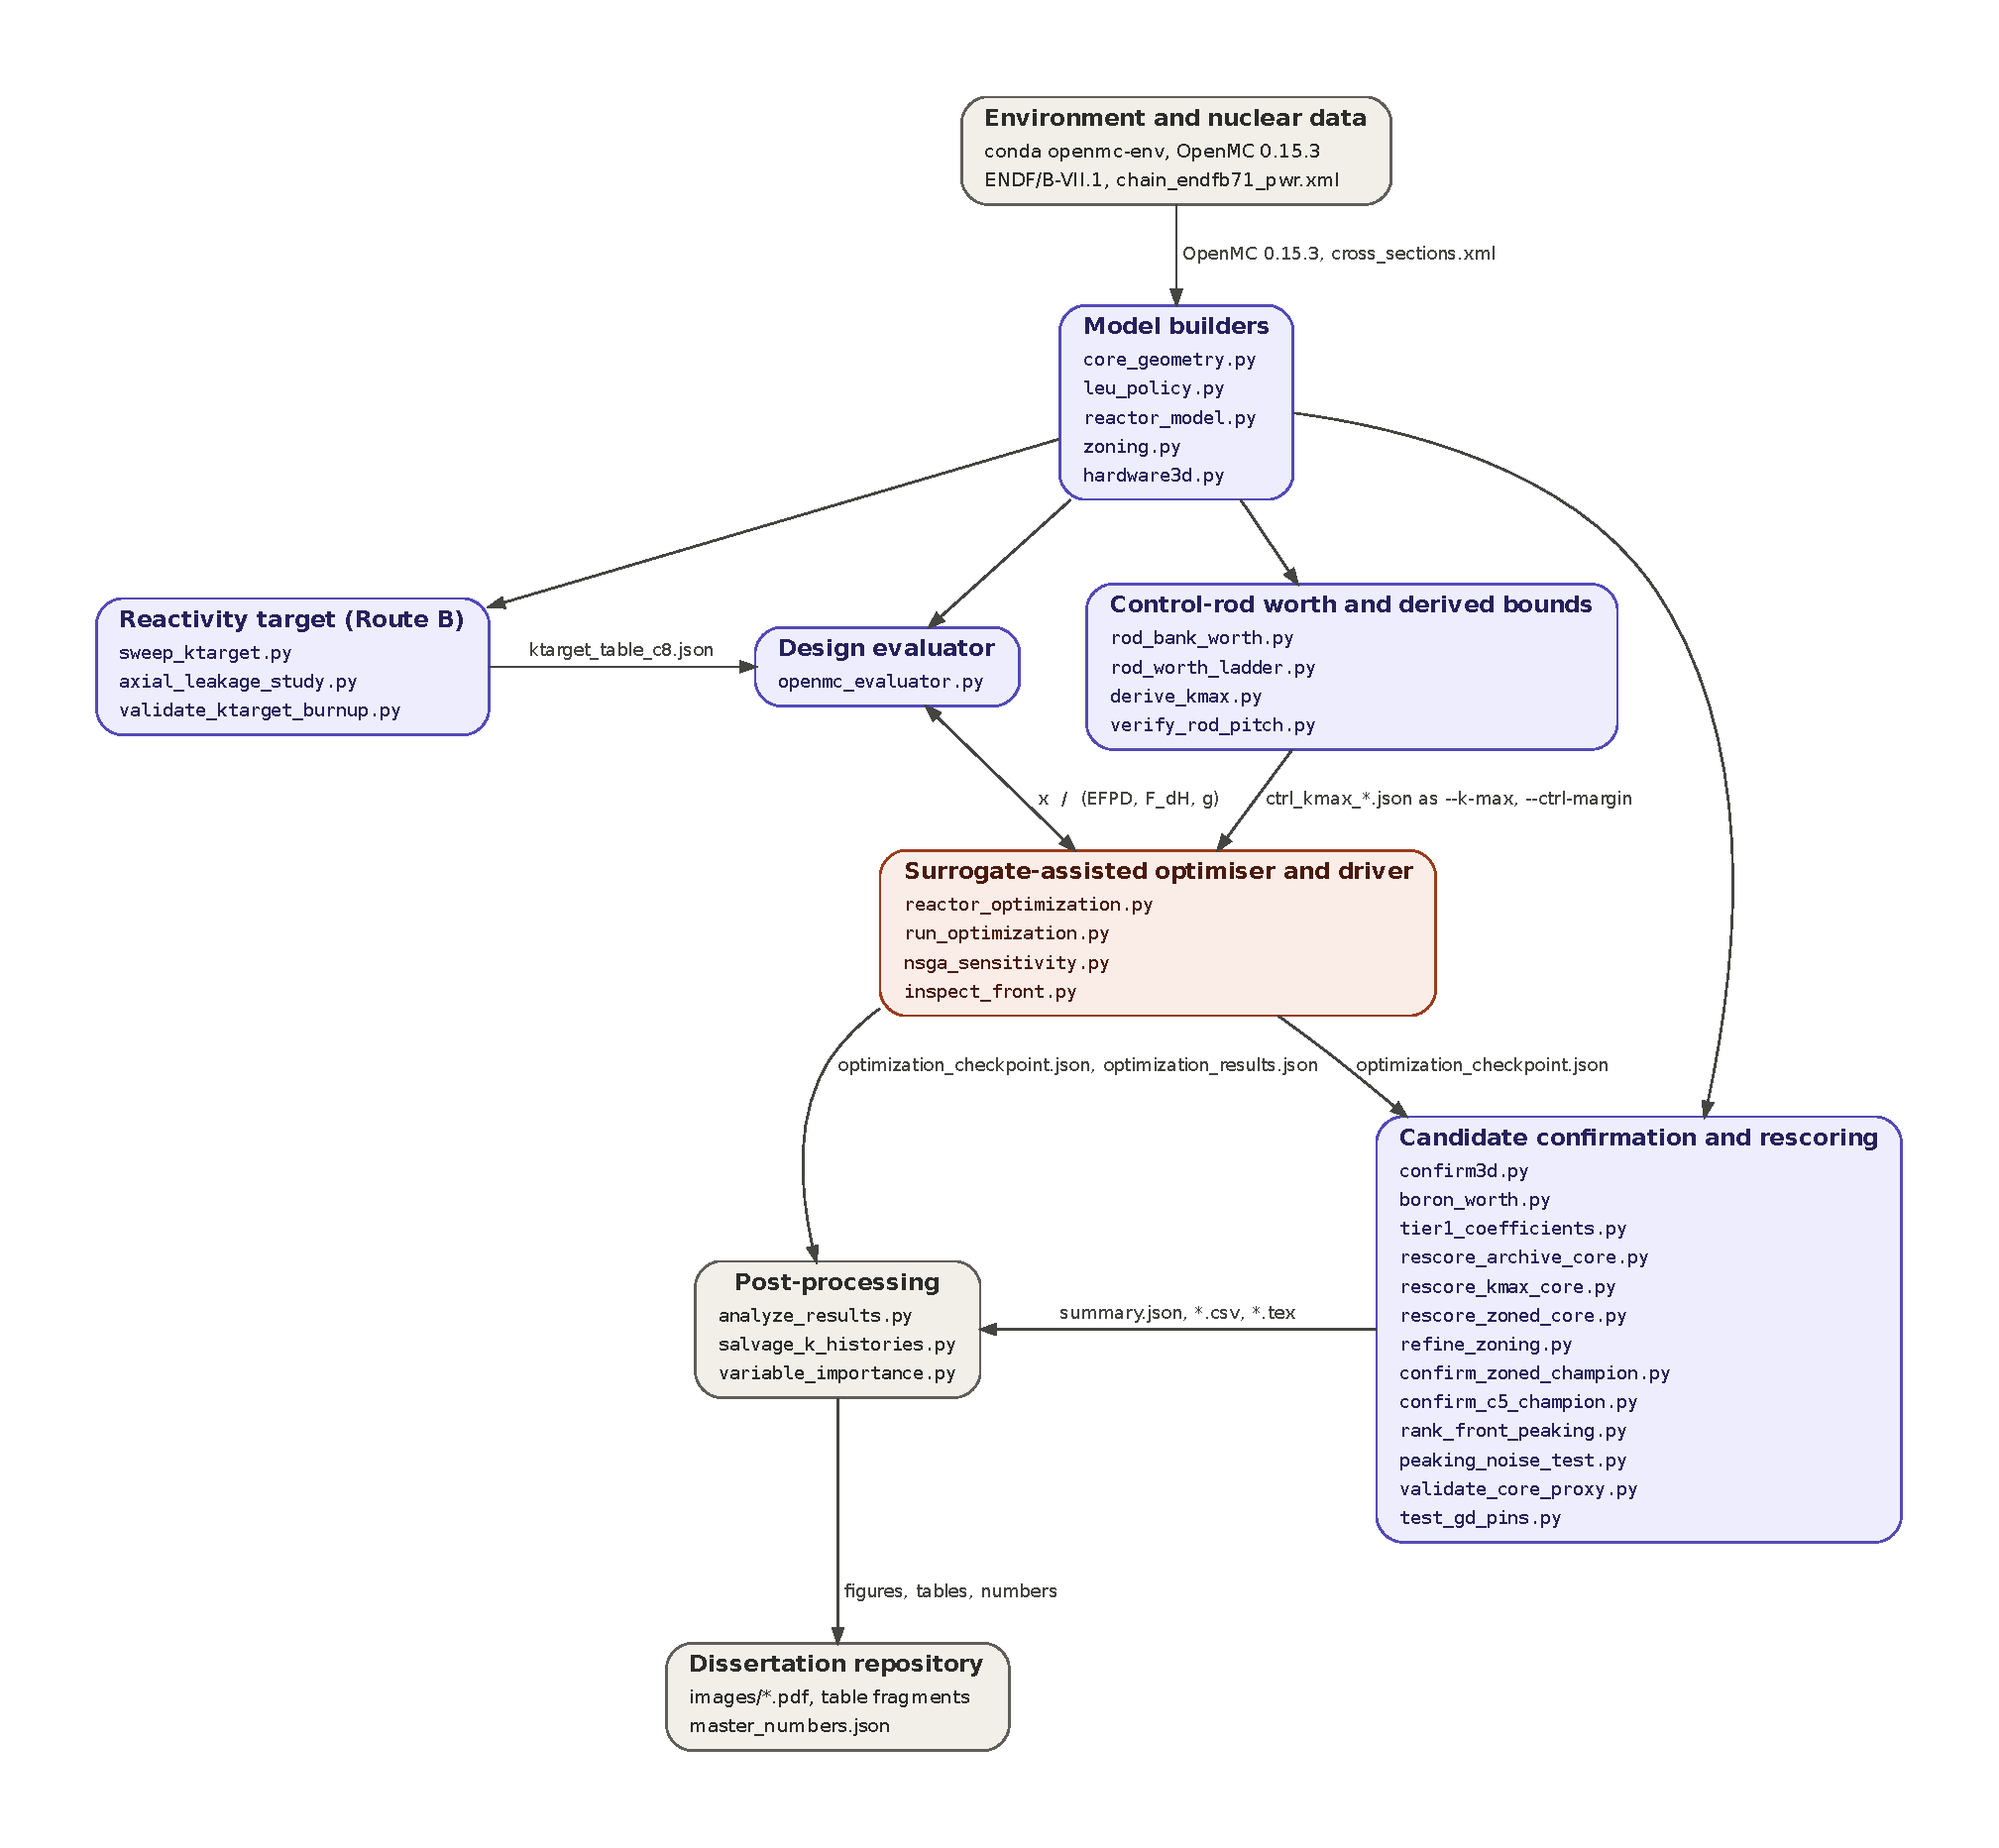
\includegraphics[width=\linewidth]{images/code_architecture.pdf}
  \caption{Macro architecture of the simulation code. Purple blocks run
  OpenMC, the coral block runs the surrogate-assisted optimiser, gray blocks
  are infrastructure and outputs. Scripts listed inside each block are
  detailed in Tables~\ref{tab:arch-builders} to \ref{tab:arch-post}.}
  \label{fig:code-architecture}
\end{figure}

One campaign traverses the blocks in the following order.

\begin{enumerate}[nosep]
  \item The reactivity target table and the derived reactivity ceiling are
        computed once, before the campaign, by the reactivity-target block
        and the control-rod block.
  \item The driver samples the Design of Experiments (DOE) by Latin
        Hypercube Sampling (LHS) \cite{mckay_lhs_1979} and sends each design
        vector to the evaluator.
  \item The evaluator builds the OpenMC models, runs the assembly depletion
        and the core solves, and returns the objectives and the constraint
        vector.
  \item The optimiser fits the Gaussian Process (GP) surrogates
        \cite{rasmussen_gp_2006}, runs the Non-dominated Sorting Genetic
        Algorithm II (NSGA-II) \cite{deb_nsga2_2002} on the surrogates, and
        selects the infill batch. Steps 3 and 4 repeat for each block of
        iterations.
  \item The confirmation block re-evaluates the archived candidates at
        higher fidelity, in three dimensions, and with the control and boron
        studies.
  \item The post-processing block extracts the front, the hypervolume
        history and the corrected depletion histories, and feeds the
        dissertation repository.
\end{enumerate}

\section{Blocks}

\subsection{Environment and nuclear data}

All physics blocks run inside one conda environment, \texttt{openmc-env},
pinned by \texttt{environment.yml} and reproduced in a Docker image by the
\texttt{Dockerfile}. The environment provides OpenMC 0.15.3
\cite{romano_openmc_2015,romano_2021_depletion}, pymoo 0.6.2
\cite{blank_deb_2020} and scikit-learn \cite{pedregosa_sklearn_2011}.

The nuclear data are the ENDF/B-VII.1 continuous-energy cross sections
\cite{chadwick_endf71_2011} and the depletion chain
\file{chain_endfb71_pwr.xml}, downloaded once per machine by
\texttt{setup\_data.sh}. Every script resolves the cross sections through
the environment variable \texttt{OPENMC\_CROSS\_SECTIONS} and the depletion
chain through \texttt{OPENMC\_CHAIN\_FILE}, so no path is written in the
source.

\subsection{Model builders}

This block holds the five library modules that every physics script
imports. They contain no command-line interface and write no result file.
Their outputs are OpenMC model objects, built in memory from a design
dictionary.

\begin{table}[htbp]
  \centering\footnotesize
  \caption{Model builders. These modules are imported, never run.}
  \label{tab:arch-builders}
  \begin{tabularx}{\linewidth}{@{}>{\raggedright\arraybackslash}p{3.6cm} X@{}}
    \toprule
    Module & Role \\
    \midrule
    \file{core_geometry.py} & Vessel envelope, geometric margin, maximum
      reflector thickness, end-of-cycle crossing of the reactivity history,
      bilinear interpolation of the target table \\
    \file{leu_policy.py} & Enrichment cap and search-box constants, defined
      once so that the search box, the evaluator and the driver cannot
      disagree \\
    \file{reactor_model.py} & Materials, fuel pin, guide tube, control-rod
      universes, $17\times17$ assembly and 32-assembly core builders,
      gadolinium pin pattern \\
    \file{zoning.py} & Ring map, centre, middle and periphery multipliers,
      control-bank positions, core beginning-of-life solve, reactivity
      history reader \\
    \file{hardware3d.py} & Finite-height core with the assembly hardware
      stack, used by the three-dimensional confirmation \\
    \bottomrule
  \end{tabularx}
\end{table}

\subsection{Reactivity target (Route B)}

This block produces the end-of-cycle reactivity target used by the
evaluator, as described in the methodology. The target is tabulated on the
full core, corrected for axial leakage, and validated against the burnup
dependence of the leakage.

\begin{table}[htbp]
  \centering\footnotesize
  \caption{Reactivity-target block. The two validation scripts read the
  campaign checkpoint to select the designs they evaluate.}
  \label{tab:arch-ktarget}
  \begin{tabularx}{\linewidth}{@{}>{\raggedright\arraybackslash}p{5.0cm} X >{\raggedright\arraybackslash}p{4.4cm}@{}}
    \toprule
    Script & Role & Main output \\
    \midrule
    \file{sweep_ktarget.py} & Tabulates the target versus pitch and
      reflector thickness from paired assembly and core solves &
      \file{ktarget_table.json} \\
    \file{axial_leakage_study.py} & Axial leakage factor
      $L_{\mathrm{ax}} = k_{2\mathrm{D}}/k_{3\mathrm{D}}$ on archived designs &
      \file{axial_<absorber>.json} \\
    \file{validate_ktarget_burnup.py} & Burnup dependence of the target on
      the front designs & \file{summary.json} \\
    \bottomrule
  \end{tabularx}
\end{table}

\subsection{Design evaluator}

The evaluator is a single module, \file{openmc_evaluator.py}. It is the
only place where a design vector becomes physics. Its public method
\texttt{evaluate\_one} performs three solves per design and returns the
mapping

\[
  \mathbf{x} = \left(e,\, w_{\mathrm{Gd}},\, t_{\mathrm{refl}},\, n_{\mathrm{Gd}}\right)
  \quad\longmapsto\quad
  \left(T_{\mathrm{EFPD}},\, F_{\Delta H},\, \mathbf{g}\right)
\]

\begin{description}[nosep]
  \item[$e$] fuel enrichment, in weight percent of \isotope[235]{U}
  \item[$w_{\mathrm{Gd}}$] gadolinia loading of the poisoned pins, in weight percent
  \item[$t_{\mathrm{refl}}$] radial reflector thickness, in cm
  \item[$n_{\mathrm{Gd}}$] number of poisoned pins per assembly, dimensionless
  \item[$T_{\mathrm{EFPD}}$] cycle length, in effective full power days
  \item[$F_{\Delta H}$] radial enthalpy-rise hot channel factor, dimensionless
  \item[$\mathbf{g}$] constraint vector on reactivity, enrichment and controllability, each entry normalised by its own limit, dimensionless
\end{description}

The three solves are the two-dimensional assembly depletion, which gives
$T_{\mathrm{EFPD}}$ through the end-of-cycle crossing of the target, the
core beginning-of-life solve, which gives $F_{\Delta H}$ and the core
eigenvalue, and the rodded core solve, which gives the controllability
entries of $\mathbf{g}$. The evaluator reads \file{ktarget_table*.json}
and writes one \file{depletion_results.h5} per case.

\subsection{Control-rod worth and derived bounds}

This block measures the worth of the control banks on archived designs and
turns the minimum worth into the reactivity ceiling passed to the driver.
It runs before a campaign, and again on the candidates after it.

\begin{table}[htbp]
  \centering\footnotesize
  \caption{Control-rod block. All scripts read the campaign checkpoint
  except \texttt{derive\_kmax.py}, which reads the screen written by
  \texttt{rod\_bank\_worth.py}.}
  \label{tab:arch-ctrl}
  \begin{tabularx}{\linewidth}{@{}>{\raggedright\arraybackslash}p{5.0cm} X >{\raggedright\arraybackslash}p{4.4cm}@{}}
    \toprule
    Script & Role & Main output \\
    \midrule
    \file{rod_bank_worth.py} & Bank worths and controllability screen of
      archived designs & \file{banks_<absorber>.json} \\
    \file{rod_worth_ladder.py} & Rod-worth ladder and rodded peaking of the
      zoned core & \file{ladder_idx<i>_}\newline\file{<absorber>.json} \\
    \file{derive_kmax.py} & Reactivity ceiling from the minimum bank worth
      and the controllability margin & \file{ctrl_kmax_<group>.json} \\
    \file{verify_rod_pitch.py} & Guide-tube clipping study versus pin pitch &
      \file{fig_rod_pitch_*.pdf} \\
    \bottomrule
  \end{tabularx}
\end{table}

\subsection{Surrogate-assisted optimiser and driver}

The optimiser holds the design space, the surrogates, the acquisition step
and the checkpoint. The driver exposes it as a command line, records the
provenance of every run in the checkpoint, and refuses to resume a
checkpoint whose settings differ from the current command.

\begin{table}[htbp]
  \centering\footnotesize
  \caption{Optimiser block. The driver reads the target table and, on
  resume, the checkpoint. The two analysis scripts read the checkpoint.}
  \label{tab:arch-optimiser}
  \begin{tabularx}{\linewidth}{@{}>{\raggedright\arraybackslash}p{5.0cm} X >{\raggedright\arraybackslash}p{4.4cm}@{}}
    \toprule
    Script & Role & Main output \\
    \midrule
    \file{reactor_optimization.py} & Design space, GP surrogates, NSGA-II
      acquisition on the surrogates, feasibility margin, batch diversity,
      hypervolume, checkpoint & \file{optimization_}\newline\file{checkpoint.json} \\
    \file{run_optimization.py} & Command-line driver: DOE, blocks of infill
      iterations, resume, provenance & \file{optimization_}\newline\file{results.json} \\
    \file{nsga_sensitivity.py} & Sensitivity of the acquisition step to the
      NSGA-II population, generations and seed & \file{nsga_sensitivity.json} \\
    \file{inspect_front.py} & Census of a live checkpoint: front, screens,
      per-block diversity & \file{<prefix>_front.csv} \\
    \bottomrule
  \end{tabularx}
\end{table}

\subsection{Candidate confirmation and rescoring}

This block re-evaluates archived designs outside the optimisation loop. Its
scripts share one pattern. They read the campaign checkpoint, select
designs by index or by front membership, run OpenMC at a fidelity chosen on
the command line, cache every solve in a \file{runs.json} keyed by design
and state, and write a summary. The cache makes every script resumable.

\begin{table}[htbp]
  \centering\footnotesize
  \caption{Confirmation block. All scripts read the campaign checkpoint.}
  \label{tab:arch-confirm}
  \begin{tabularx}{\linewidth}{@{}>{\raggedright\arraybackslash}p{5.0cm} X >{\raggedright\arraybackslash}p{4.4cm}@{}}
    \toprule
    Script & Role & Main output \\
    \midrule
    \file{confirm3d.py} & Three-dimensional confirmation with the hardware
      stack, several rod states and boron concentrations & \file{summary.json} \\
    \file{boron_worth.py} & Boron worth and share of the beginning-of-life
      hold-down across rod states and concentrations & \file{boron_table.tex} \\
    \file{tier1_coefficients.py} & Reactivity coefficients of a candidate &
      \file{tier1_idx<i>.json} \\
    \file{rescore_archive_core.py} & Core-basis peaking of an assembly-basis
      archive & \file{core_rescore.csv} \\
    \file{rescore_kmax_core.py} & Re-screens a finished campaign on the core
      reactivity limits & \file{<label>_kbasis_}\newline\file{summary.json} \\
    \file{rescore_zoned_core.py} & Transfer test of the zoned loading on an
      archive & \file{transfer_summary.json} \\
    \file{refine_zoning.py} & Refinement of the ring multipliers of a
      champion & \file{runs.json} \\
    \file{confirm_zoned_champion.py} & Depletion of the zoned champion at
      full fidelity & \file{confirm_idx<i>.json} \\
    \file{confirm_c5_champion.py} & Feasibility of the Campaign 5 champion
      at full fidelity & \file{summary.json} \\
    \file{rank_front_peaking.py} & Minimum-$F_{\Delta H}$ design beyond
      Monte Carlo noise, by sequential screening & \file{ranking.csv} \\
    \file{peaking_noise_test.py} & Seed replicates of $F_{\Delta H}$ on the
      front designs & \file{noise_summary.csv} \\
    \file{validate_core_proxy.py} & Assembly-to-core peaking proxy
      validation & \file{core_validation.csv} \\
    \file{test_gd_pins.py} & Gadolinium pin-count test on a champion,
      assembly and core & \file{summary.json} \\
    \bottomrule
  \end{tabularx}
\end{table}

\subsection{Post-processing}

The post-processing block reads the campaign archive and the confirmation
summaries and produces the quantities reported in the results chapters.

\begin{table}[htbp]
  \centering\footnotesize
  \caption{Post-processing block. Figure generators and log parsers are
  omitted, see Section~\ref{sec:arch-scope}.}
  \label{tab:arch-post}
  \begin{tabularx}{\linewidth}{@{}>{\raggedright\arraybackslash}p{5.0cm} X >{\raggedright\arraybackslash}p{4.4cm}@{}}
    \toprule
    Script & Role & Main output \\
    \midrule
    \file{analyze_results.py} & Pareto front, hypervolume history,
      design-space diagnostics & figures \\
    \file{salvage_k_histories.py} & Corrects the archived depletion histories
      for the restart defect of the depletion chunks & \file{salvage_summary.csv} \\
    \file{variable_importance.py} & Permutation importance of the design
      variables on the archive & standard output \\
    \bottomrule
  \end{tabularx}
\end{table}

\subsection{Dissertation repository}

The dissertation is kept in a second repository,
\url{https://github.com/dcrlopes/Masther-Thesis-UNIPI---Di-go-Lopes},
synchronised with Overleaf. Figures are stored under \texttt{images/}.
Every number quoted in the text is taken from
\file{master_numbers.json}, which is the single source of truth for the
thesis.

\openpoint{\file{master_numbers.json} is not under version control in
either repository. It was produced with the computational-cost section and
lives only on the workstation. Commit it to \texttt{results\_timing/} in the
simulation repository before submission, so that the last arrow of
Figure~\ref{fig:code-architecture} points to a file a reader can open.}

\section{Interfaces between blocks}

Table~\ref{tab:arch-interfaces} lists the artefacts that cross the block
boundaries of Figure~\ref{fig:code-architecture}. Every artefact is a
plain text file, JSON or CSV, so that any stage can be inspected without
the code.

\begin{table}[htbp]
  \centering\footnotesize
  \caption{Artefacts exchanged between blocks.}
  \label{tab:arch-interfaces}
  \begin{tabularx}{\linewidth}{@{}>{\raggedright\arraybackslash}p{5.1cm} >{\raggedright\arraybackslash}p{2.1cm} >{\raggedright\arraybackslash}p{2.5cm} X@{}}
    \toprule
    Artefact & Producer & Consumer & Content \\
    \midrule
    \file{ktarget_table_c8.json} & Reactivity target & Evaluator &
      Target $k$ versus pitch and reflector thickness, with the axial
      correction $L_{\mathrm{ax}}$ \\
    \file{ctrl_kmax_<group>.json} & Control-rod worth & Driver &
      Derived ceiling, passed as \texttt{--k-max} and \texttt{--ctrl-margin} \\
    design vector $\mathbf{x}$ & Optimiser & Evaluator &
      One design per call \\
    $(T_{\mathrm{EFPD}}, F_{\Delta H}, \mathbf{g})$ & Evaluator & Optimiser &
      Objectives and normalised constraints \\
    \file{optimization_checkpoint.json} & Optimiser & Confirmation,
      post-processing & Every evaluation of the campaign with its
      provenance \\
    \file{optimization_results.json} & Optimiser & Post-processing &
      Front, raw objectives, hypervolume history \\
    \file{summary.json}, \file{*.csv} & Confirmation & Post-processing &
      Per-design results of each confirmation study \\
    \file{images/*.pdf}, \file{*.tex} & Post-processing & Dissertation &
      Figures and table fragments \\
    \bottomrule
  \end{tabularx}
\end{table}

The checkpoint is the central artefact. It is written at the end of every
block of iterations and it records the design space, the constraint
definition, the transport fidelity, the target table and the command line.
A resumed run compares these fields with its own arguments and warns on any
difference. All confirmation and post-processing scripts read the
checkpoint, never the raw case directories, so a campaign can be
re-analysed from a single file.

\openpoint{Regenerate the table of Section~1 of the repository
\texttt{README.md} with \texttt{make\_architecture\_figure.py --table md},
because the current table describes the Campaign 3 layout.}
                       (add this line)
%%   \end{appendices}
%%
%% Figure: images/code_architecture.pdf, produced by
%% make_architecture_figure.py in the simulation repository. Regenerate the
%% figure and the table rows (--table latex) whenever a script is added.
%%
%% New bibliography entries required (appended to references_additions.bib):
%%   pedregosa_sklearn_2011, chadwick_endf71_2011
%% ---------------------------------------------------------------------

\chapter{Architecture of the simulation code}\label{app:code-architecture}

\providecommand{\file}[1]{\texttt{\detokenize{#1}}}

\providecommand{\openpoint}[1]{\par\noindent\fbox{\parbox{0.97\linewidth}{%
  \small\textbf{Open point.} #1}}\par}

\section{Purpose and scope}\label{sec:arch-scope}

This appendix documents the organisation of the code that produced every
result in this thesis. It is written for a reader who needs to locate the
script behind a number, reproduce a campaign, or extend the pipeline to
another core.

The code is public. It is hosted at
\url{https://github.com/dcrlopes/master-thesis-unipi}, on the branch
\texttt{campaign8}, which is the state used for the final campaign and for
the candidate confirmation runs. The state described in this appendix is
commit \texttt{22bad3d} of 3 September 2026.

\openpoint{Update the commit hash above to the final state of branch
\texttt{campaign8} at submission. The branch \texttt{main} still holds the
Campaign 3 state of the code and must not be cited.}

The repository contains 92 Python scripts and 8 shell wrappers. Only the
scripts that perform a computation reported in the thesis are described
here. The following groups are omitted on purpose.

\begin{itemize}[nosep]
  \item Shell wrappers for launch, resume and monitoring.
  \item Anchor-verified patch scripts (\texttt{apply\_*.py},
        \texttt{fix\_*.py}, \texttt{repair\_*.py}) that modified the source
        between campaigns. Their role is described in the methodology.
  \item Figure generators, log parsers and timing accounting scripts.
  \item Unit tests, diagnostics and scripts superseded by a later version.
\end{itemize}

\section{Macro architecture}

Figure~\ref{fig:code-architecture} shows the nine blocks of the pipeline and
the artefacts that cross each interface. Purple blocks call OpenMC
\cite{romano_openmc_2015}, the Monte Carlo transport and depletion code.
The coral block is the only one that never calls OpenMC directly. Gray
blocks are infrastructure and outputs. Unlabelled arrows are Python
imports. Labelled arrows name the file, or the pair of vectors, exchanged.

\begin{figure}[htbp]
  \centering
  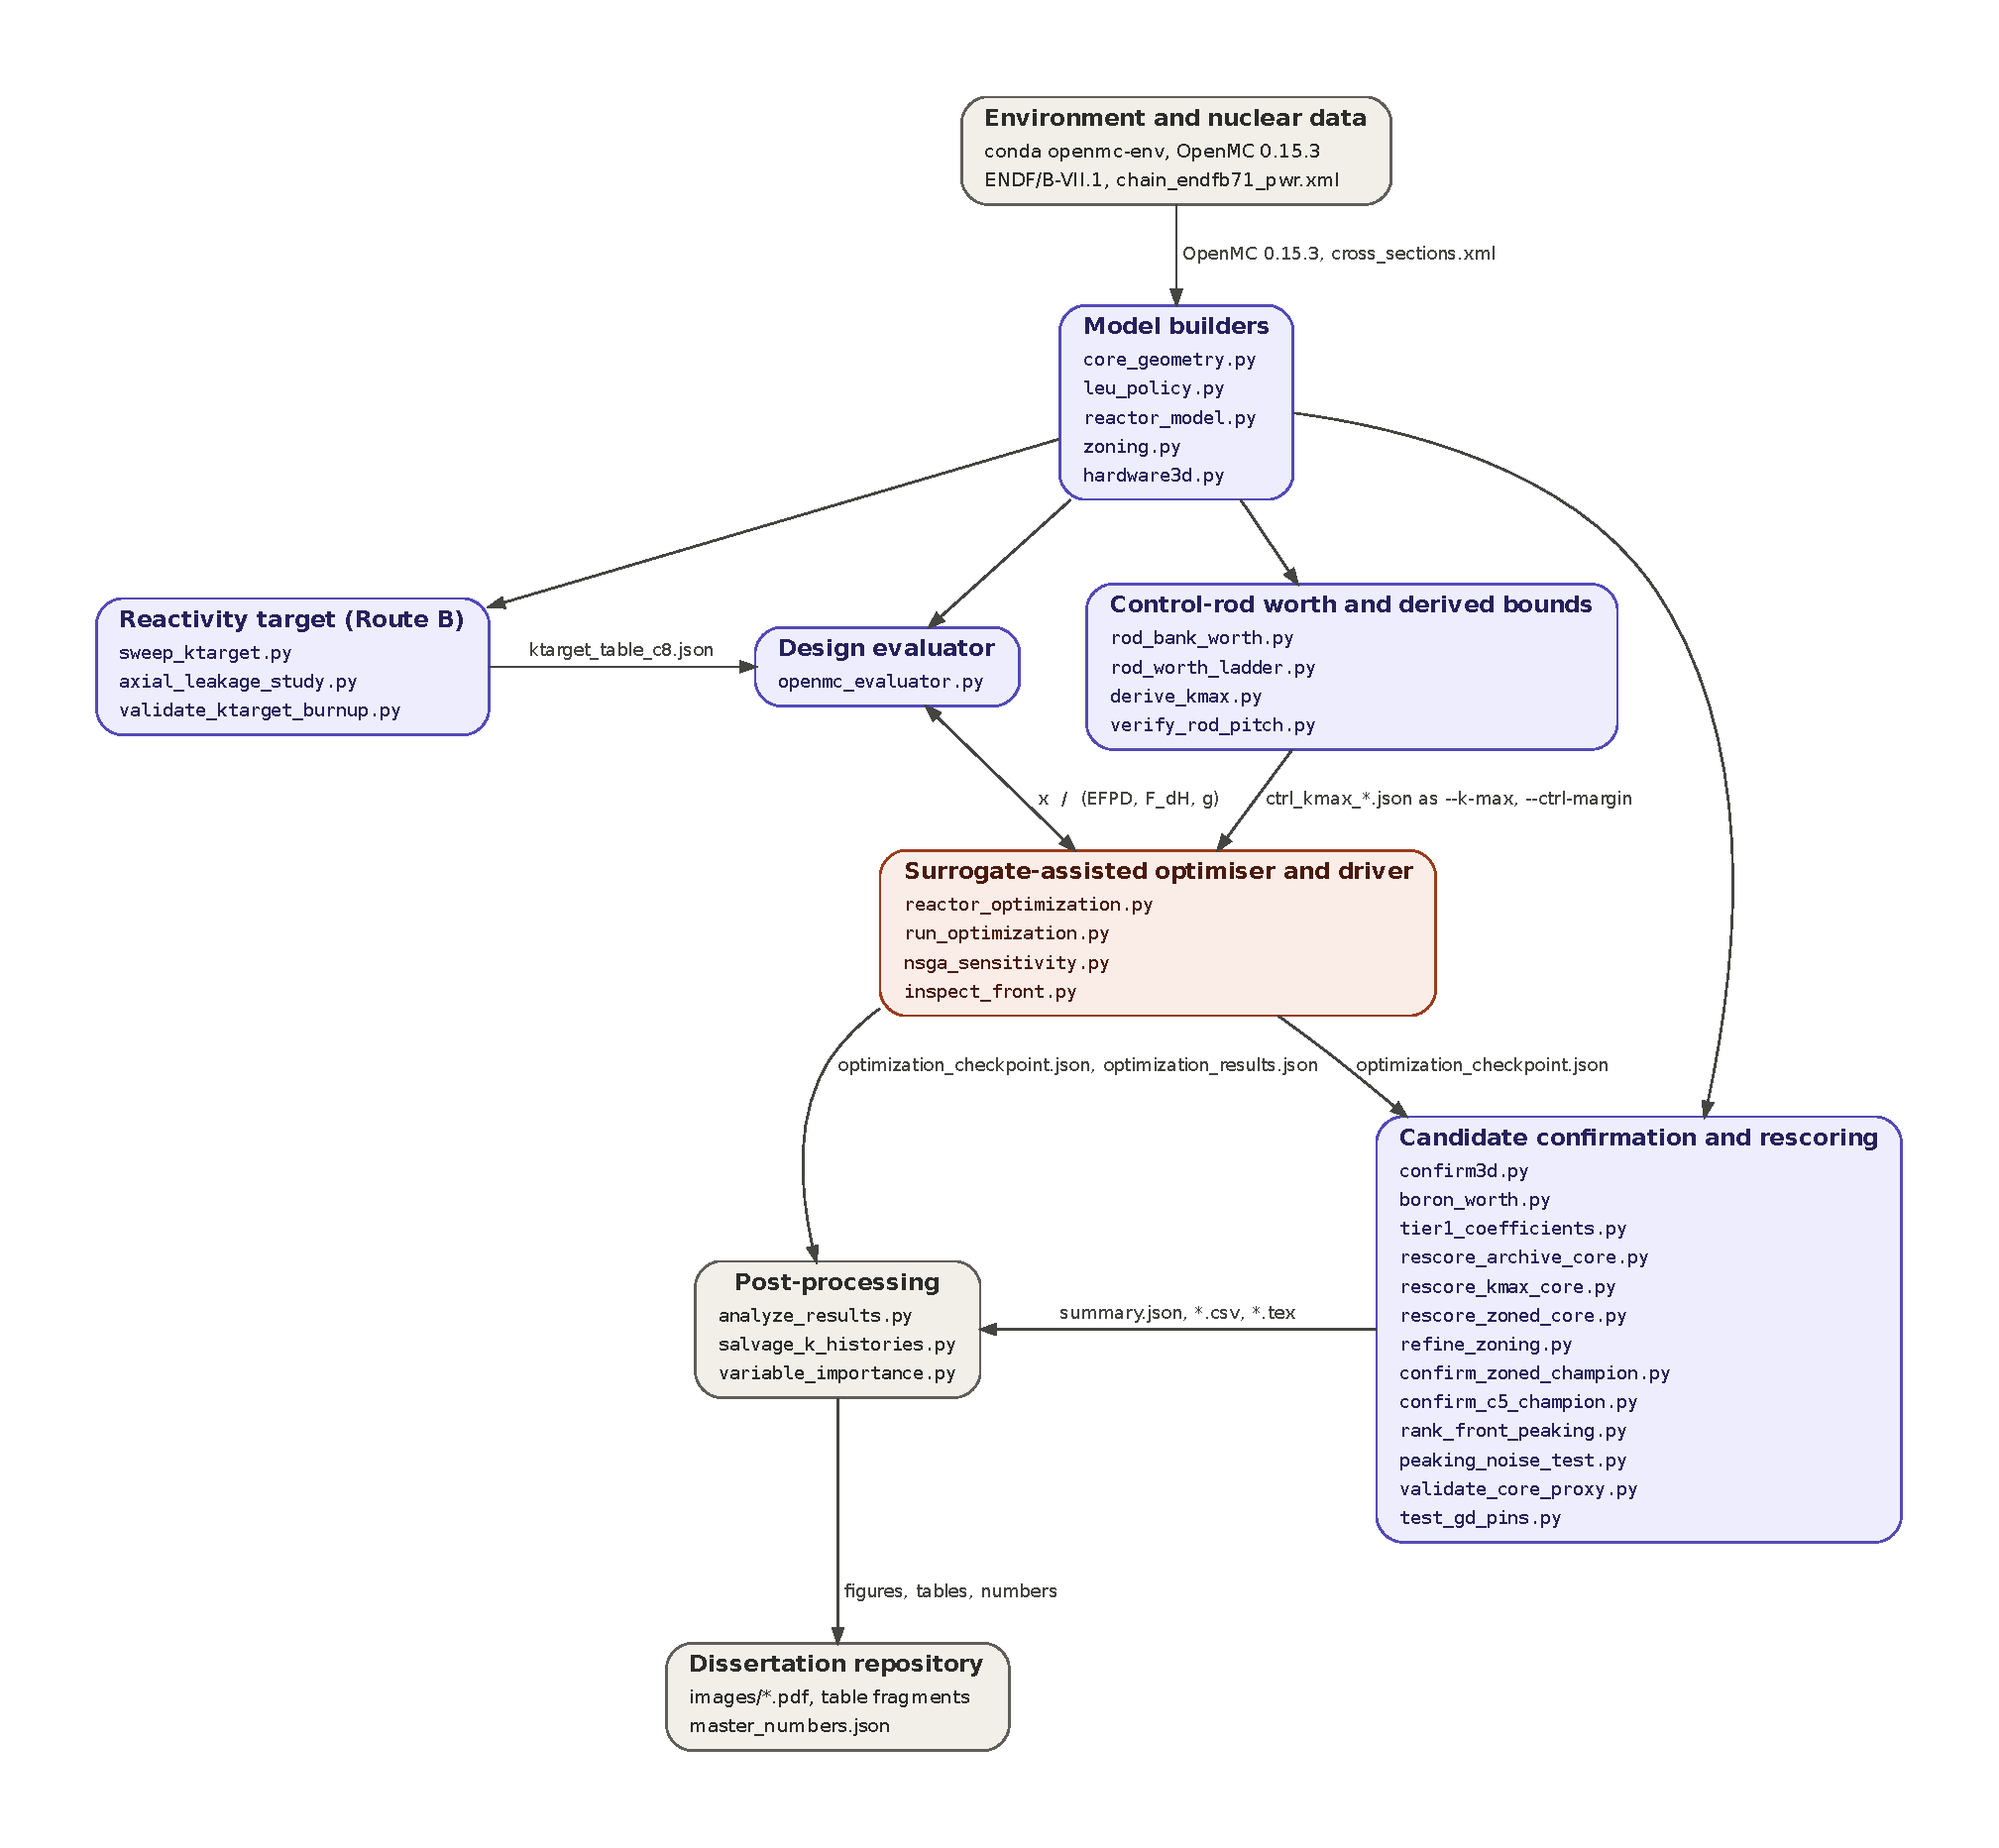
\includegraphics[width=\linewidth]{images/code_architecture.pdf}
  \caption{Macro architecture of the simulation code. Purple blocks run
  OpenMC, the coral block runs the surrogate-assisted optimiser, gray blocks
  are infrastructure and outputs. Scripts listed inside each block are
  detailed in Tables~\ref{tab:arch-builders} to \ref{tab:arch-post}.}
  \label{fig:code-architecture}
\end{figure}

One campaign traverses the blocks in the following order.

\begin{enumerate}[nosep]
  \item The reactivity target table and the derived reactivity ceiling are
        computed once, before the campaign, by the reactivity-target block
        and the control-rod block.
  \item The driver samples the Design of Experiments (DOE) by Latin
        Hypercube Sampling (LHS) \cite{mckay_lhs_1979} and sends each design
        vector to the evaluator.
  \item The evaluator builds the OpenMC models, runs the assembly depletion
        and the core solves, and returns the objectives and the constraint
        vector.
  \item The optimiser fits the Gaussian Process (GP) surrogates
        \cite{rasmussen_gp_2006}, runs the Non-dominated Sorting Genetic
        Algorithm II (NSGA-II) \cite{deb_nsga2_2002} on the surrogates, and
        selects the infill batch. Steps 3 and 4 repeat for each block of
        iterations.
  \item The confirmation block re-evaluates the archived candidates at
        higher fidelity, in three dimensions, and with the control and boron
        studies.
  \item The post-processing block extracts the front, the hypervolume
        history and the corrected depletion histories, and feeds the
        dissertation repository.
\end{enumerate}

\section{Blocks}

\subsection{Environment and nuclear data}

All physics blocks run inside one conda environment, \texttt{openmc-env},
pinned by \texttt{environment.yml} and reproduced in a Docker image by the
\texttt{Dockerfile}. The environment provides OpenMC 0.15.3
\cite{romano_openmc_2015,romano_2021_depletion}, pymoo 0.6.2
\cite{blank_deb_2020} and scikit-learn \cite{pedregosa_sklearn_2011}.

The nuclear data are the ENDF/B-VII.1 continuous-energy cross sections
\cite{chadwick_endf71_2011} and the depletion chain
\file{chain_endfb71_pwr.xml}, downloaded once per machine by
\texttt{setup\_data.sh}. Every script resolves the cross sections through
the environment variable \texttt{OPENMC\_CROSS\_SECTIONS} and the depletion
chain through \texttt{OPENMC\_CHAIN\_FILE}, so no path is written in the
source.

\subsection{Model builders}

This block holds the five library modules that every physics script
imports. They contain no command-line interface and write no result file.
Their outputs are OpenMC model objects, built in memory from a design
dictionary.

\begin{table}[htbp]
  \centering\footnotesize
  \caption{Model builders. These modules are imported, never run.}
  \label{tab:arch-builders}
  \begin{tabularx}{\linewidth}{@{}>{\raggedright\arraybackslash}p{3.6cm} X@{}}
    \toprule
    Module & Role \\
    \midrule
    \file{core_geometry.py} & Vessel envelope, geometric margin, maximum
      reflector thickness, end-of-cycle crossing of the reactivity history,
      bilinear interpolation of the target table \\
    \file{leu_policy.py} & Enrichment cap and search-box constants, defined
      once so that the search box, the evaluator and the driver cannot
      disagree \\
    \file{reactor_model.py} & Materials, fuel pin, guide tube, control-rod
      universes, $17\times17$ assembly and 32-assembly core builders,
      gadolinium pin pattern \\
    \file{zoning.py} & Ring map, centre, middle and periphery multipliers,
      control-bank positions, core beginning-of-life solve, reactivity
      history reader \\
    \file{hardware3d.py} & Finite-height core with the assembly hardware
      stack, used by the three-dimensional confirmation \\
    \bottomrule
  \end{tabularx}
\end{table}

\subsection{Reactivity target (Route B)}

This block produces the end-of-cycle reactivity target used by the
evaluator, as described in the methodology. The target is tabulated on the
full core, corrected for axial leakage, and validated against the burnup
dependence of the leakage.

\begin{table}[htbp]
  \centering\footnotesize
  \caption{Reactivity-target block. The two validation scripts read the
  campaign checkpoint to select the designs they evaluate.}
  \label{tab:arch-ktarget}
  \begin{tabularx}{\linewidth}{@{}>{\raggedright\arraybackslash}p{5.0cm} X >{\raggedright\arraybackslash}p{4.4cm}@{}}
    \toprule
    Script & Role & Main output \\
    \midrule
    \file{sweep_ktarget.py} & Tabulates the target versus pitch and
      reflector thickness from paired assembly and core solves &
      \file{ktarget_table.json} \\
    \file{axial_leakage_study.py} & Axial leakage factor
      $L_{\mathrm{ax}} = k_{2\mathrm{D}}/k_{3\mathrm{D}}$ on archived designs &
      \file{axial_<absorber>.json} \\
    \file{validate_ktarget_burnup.py} & Burnup dependence of the target on
      the front designs & \file{summary.json} \\
    \bottomrule
  \end{tabularx}
\end{table}

\subsection{Design evaluator}

The evaluator is a single module, \file{openmc_evaluator.py}. It is the
only place where a design vector becomes physics. Its public method
\texttt{evaluate\_one} performs three solves per design and returns the
mapping

\[
  \mathbf{x} = \left(e,\, w_{\mathrm{Gd}},\, t_{\mathrm{refl}},\, n_{\mathrm{Gd}}\right)
  \quad\longmapsto\quad
  \left(T_{\mathrm{EFPD}},\, F_{\Delta H},\, \mathbf{g}\right)
\]

\begin{description}[nosep]
  \item[$e$] fuel enrichment, in weight percent of \isotope[235]{U}
  \item[$w_{\mathrm{Gd}}$] gadolinia loading of the poisoned pins, in weight percent
  \item[$t_{\mathrm{refl}}$] radial reflector thickness, in cm
  \item[$n_{\mathrm{Gd}}$] number of poisoned pins per assembly, dimensionless
  \item[$T_{\mathrm{EFPD}}$] cycle length, in effective full power days
  \item[$F_{\Delta H}$] radial enthalpy-rise hot channel factor, dimensionless
  \item[$\mathbf{g}$] constraint vector on reactivity, enrichment and controllability, each entry normalised by its own limit, dimensionless
\end{description}

The three solves are the two-dimensional assembly depletion, which gives
$T_{\mathrm{EFPD}}$ through the end-of-cycle crossing of the target, the
core beginning-of-life solve, which gives $F_{\Delta H}$ and the core
eigenvalue, and the rodded core solve, which gives the controllability
entries of $\mathbf{g}$. The evaluator reads \file{ktarget_table*.json}
and writes one \file{depletion_results.h5} per case.

\subsection{Control-rod worth and derived bounds}

This block measures the worth of the control banks on archived designs and
turns the minimum worth into the reactivity ceiling passed to the driver.
It runs before a campaign, and again on the candidates after it.

\begin{table}[htbp]
  \centering\footnotesize
  \caption{Control-rod block. All scripts read the campaign checkpoint
  except \texttt{derive\_kmax.py}, which reads the screen written by
  \texttt{rod\_bank\_worth.py}.}
  \label{tab:arch-ctrl}
  \begin{tabularx}{\linewidth}{@{}>{\raggedright\arraybackslash}p{5.0cm} X >{\raggedright\arraybackslash}p{4.4cm}@{}}
    \toprule
    Script & Role & Main output \\
    \midrule
    \file{rod_bank_worth.py} & Bank worths and controllability screen of
      archived designs & \file{banks_<absorber>.json} \\
    \file{rod_worth_ladder.py} & Rod-worth ladder and rodded peaking of the
      zoned core & \file{ladder_idx<i>_}\newline\file{<absorber>.json} \\
    \file{derive_kmax.py} & Reactivity ceiling from the minimum bank worth
      and the controllability margin & \file{ctrl_kmax_<group>.json} \\
    \file{verify_rod_pitch.py} & Guide-tube clipping study versus pin pitch &
      \file{fig_rod_pitch_*.pdf} \\
    \bottomrule
  \end{tabularx}
\end{table}

\subsection{Surrogate-assisted optimiser and driver}

The optimiser holds the design space, the surrogates, the acquisition step
and the checkpoint. The driver exposes it as a command line, records the
provenance of every run in the checkpoint, and refuses to resume a
checkpoint whose settings differ from the current command.

\begin{table}[htbp]
  \centering\footnotesize
  \caption{Optimiser block. The driver reads the target table and, on
  resume, the checkpoint. The two analysis scripts read the checkpoint.}
  \label{tab:arch-optimiser}
  \begin{tabularx}{\linewidth}{@{}>{\raggedright\arraybackslash}p{5.0cm} X >{\raggedright\arraybackslash}p{4.4cm}@{}}
    \toprule
    Script & Role & Main output \\
    \midrule
    \file{reactor_optimization.py} & Design space, GP surrogates, NSGA-II
      acquisition on the surrogates, feasibility margin, batch diversity,
      hypervolume, checkpoint & \file{optimization_}\newline\file{checkpoint.json} \\
    \file{run_optimization.py} & Command-line driver: DOE, blocks of infill
      iterations, resume, provenance & \file{optimization_}\newline\file{results.json} \\
    \file{nsga_sensitivity.py} & Sensitivity of the acquisition step to the
      NSGA-II population, generations and seed & \file{nsga_sensitivity.json} \\
    \file{inspect_front.py} & Census of a live checkpoint: front, screens,
      per-block diversity & \file{<prefix>_front.csv} \\
    \bottomrule
  \end{tabularx}
\end{table}

\subsection{Candidate confirmation and rescoring}

This block re-evaluates archived designs outside the optimisation loop. Its
scripts share one pattern. They read the campaign checkpoint, select
designs by index or by front membership, run OpenMC at a fidelity chosen on
the command line, cache every solve in a \file{runs.json} keyed by design
and state, and write a summary. The cache makes every script resumable.

\begin{table}[htbp]
  \centering\footnotesize
  \caption{Confirmation block. All scripts read the campaign checkpoint.}
  \label{tab:arch-confirm}
  \begin{tabularx}{\linewidth}{@{}>{\raggedright\arraybackslash}p{5.0cm} X >{\raggedright\arraybackslash}p{4.4cm}@{}}
    \toprule
    Script & Role & Main output \\
    \midrule
    \file{confirm3d.py} & Three-dimensional confirmation with the hardware
      stack, several rod states and boron concentrations & \file{summary.json} \\
    \file{boron_worth.py} & Boron worth and share of the beginning-of-life
      hold-down across rod states and concentrations & \file{boron_table.tex} \\
    \file{tier1_coefficients.py} & Reactivity coefficients of a candidate &
      \file{tier1_idx<i>.json} \\
    \file{rescore_archive_core.py} & Core-basis peaking of an assembly-basis
      archive & \file{core_rescore.csv} \\
    \file{rescore_kmax_core.py} & Re-screens a finished campaign on the core
      reactivity limits & \file{<label>_kbasis_}\newline\file{summary.json} \\
    \file{rescore_zoned_core.py} & Transfer test of the zoned loading on an
      archive & \file{transfer_summary.json} \\
    \file{refine_zoning.py} & Refinement of the ring multipliers of a
      champion & \file{runs.json} \\
    \file{confirm_zoned_champion.py} & Depletion of the zoned champion at
      full fidelity & \file{confirm_idx<i>.json} \\
    \file{confirm_c5_champion.py} & Feasibility of the Campaign 5 champion
      at full fidelity & \file{summary.json} \\
    \file{rank_front_peaking.py} & Minimum-$F_{\Delta H}$ design beyond
      Monte Carlo noise, by sequential screening & \file{ranking.csv} \\
    \file{peaking_noise_test.py} & Seed replicates of $F_{\Delta H}$ on the
      front designs & \file{noise_summary.csv} \\
    \file{validate_core_proxy.py} & Assembly-to-core peaking proxy
      validation & \file{core_validation.csv} \\
    \file{test_gd_pins.py} & Gadolinium pin-count test on a champion,
      assembly and core & \file{summary.json} \\
    \bottomrule
  \end{tabularx}
\end{table}

\subsection{Post-processing}

The post-processing block reads the campaign archive and the confirmation
summaries and produces the quantities reported in the results chapters.

\begin{table}[htbp]
  \centering\footnotesize
  \caption{Post-processing block. Figure generators and log parsers are
  omitted, see Section~\ref{sec:arch-scope}.}
  \label{tab:arch-post}
  \begin{tabularx}{\linewidth}{@{}>{\raggedright\arraybackslash}p{5.0cm} X >{\raggedright\arraybackslash}p{4.4cm}@{}}
    \toprule
    Script & Role & Main output \\
    \midrule
    \file{analyze_results.py} & Pareto front, hypervolume history,
      design-space diagnostics & figures \\
    \file{salvage_k_histories.py} & Corrects the archived depletion histories
      for the restart defect of the depletion chunks & \file{salvage_summary.csv} \\
    \file{variable_importance.py} & Permutation importance of the design
      variables on the archive & standard output \\
    \bottomrule
  \end{tabularx}
\end{table}

\subsection{Dissertation repository}

The dissertation is kept in a second repository,
\url{https://github.com/dcrlopes/Masther-Thesis-UNIPI---Di-go-Lopes},
synchronised with Overleaf. Figures are stored under \texttt{images/}.
Every number quoted in the text is taken from
\file{master_numbers.json}, which is the single source of truth for the
thesis.

\openpoint{\file{master_numbers.json} is not under version control in
either repository. It was produced with the computational-cost section and
lives only on the workstation. Commit it to \texttt{results\_timing/} in the
simulation repository before submission, so that the last arrow of
Figure~\ref{fig:code-architecture} points to a file a reader can open.}

\section{Interfaces between blocks}

Table~\ref{tab:arch-interfaces} lists the artefacts that cross the block
boundaries of Figure~\ref{fig:code-architecture}. Every artefact is a
plain text file, JSON or CSV, so that any stage can be inspected without
the code.

\begin{table}[htbp]
  \centering\footnotesize
  \caption{Artefacts exchanged between blocks.}
  \label{tab:arch-interfaces}
  \begin{tabularx}{\linewidth}{@{}>{\raggedright\arraybackslash}p{5.1cm} >{\raggedright\arraybackslash}p{2.1cm} >{\raggedright\arraybackslash}p{2.5cm} X@{}}
    \toprule
    Artefact & Producer & Consumer & Content \\
    \midrule
    \file{ktarget_table_c8.json} & Reactivity target & Evaluator &
      Target $k$ versus pitch and reflector thickness, with the axial
      correction $L_{\mathrm{ax}}$ \\
    \file{ctrl_kmax_<group>.json} & Control-rod worth & Driver &
      Derived ceiling, passed as \texttt{--k-max} and \texttt{--ctrl-margin} \\
    design vector $\mathbf{x}$ & Optimiser & Evaluator &
      One design per call \\
    $(T_{\mathrm{EFPD}}, F_{\Delta H}, \mathbf{g})$ & Evaluator & Optimiser &
      Objectives and normalised constraints \\
    \file{optimization_checkpoint.json} & Optimiser & Confirmation,
      post-processing & Every evaluation of the campaign with its
      provenance \\
    \file{optimization_results.json} & Optimiser & Post-processing &
      Front, raw objectives, hypervolume history \\
    \file{summary.json}, \file{*.csv} & Confirmation & Post-processing &
      Per-design results of each confirmation study \\
    \file{images/*.pdf}, \file{*.tex} & Post-processing & Dissertation &
      Figures and table fragments \\
    \bottomrule
  \end{tabularx}
\end{table}

The checkpoint is the central artefact. It is written at the end of every
block of iterations and it records the design space, the constraint
definition, the transport fidelity, the target table and the command line.
A resumed run compares these fields with its own arguments and warns on any
difference. All confirmation and post-processing scripts read the
checkpoint, never the raw case directories, so a campaign can be
re-analysed from a single file.

\openpoint{Regenerate the table of Section~1 of the repository
\texttt{README.md} with \texttt{make\_architecture\_figure.py --table md},
because the current table describes the Campaign 3 layout.}
                       (add this line)
%%   \end{appendices}
%%
%% Figure: images/code_architecture.pdf, produced by
%% make_architecture_figure.py in the simulation repository. Regenerate the
%% figure and the table rows (--table latex) whenever a script is added.
%%
%% New bibliography entries required (appended to references_additions.bib):
%%   pedregosa_sklearn_2011, chadwick_endf71_2011
%% ---------------------------------------------------------------------

\chapter{Architecture of the simulation code}\label{app:code-architecture}

\providecommand{\file}[1]{\texttt{\detokenize{#1}}}

\providecommand{\openpoint}[1]{\par\noindent\fbox{\parbox{0.97\linewidth}{%
  \small\textbf{Open point.} #1}}\par}

\section{Purpose and scope}\label{sec:arch-scope}

This appendix documents the organisation of the code that produced every
result in this thesis. It is written for a reader who needs to locate the
script behind a number, reproduce a campaign, or extend the pipeline to
another core.

The code is public. It is hosted at
\url{https://github.com/dcrlopes/master-thesis-unipi}, on the branch
\texttt{campaign8}, which is the state used for the final campaign and for
the candidate confirmation runs. The state described in this appendix is
commit \texttt{22bad3d} of 3 September 2026.

\openpoint{Update the commit hash above to the final state of branch
\texttt{campaign8} at submission. The branch \texttt{main} still holds the
Campaign 3 state of the code and must not be cited.}

The repository contains 92 Python scripts and 8 shell wrappers. Only the
scripts that perform a computation reported in the thesis are described
here. The following groups are omitted on purpose.

\begin{itemize}[nosep]
  \item Shell wrappers for launch, resume and monitoring.
  \item Anchor-verified patch scripts (\texttt{apply\_*.py},
        \texttt{fix\_*.py}, \texttt{repair\_*.py}) that modified the source
        between campaigns. Their role is described in the methodology.
  \item Figure generators, log parsers and timing accounting scripts.
  \item Unit tests, diagnostics and scripts superseded by a later version.
\end{itemize}

\section{Macro architecture}

Figure~\ref{fig:code-architecture} shows the nine blocks of the pipeline and
the artefacts that cross each interface. Purple blocks call OpenMC
\cite{romano_openmc_2015}, the Monte Carlo transport and depletion code.
The coral block is the only one that never calls OpenMC directly. Gray
blocks are infrastructure and outputs. Unlabelled arrows are Python
imports. Labelled arrows name the file, or the pair of vectors, exchanged.

\begin{figure}[htbp]
  \centering
  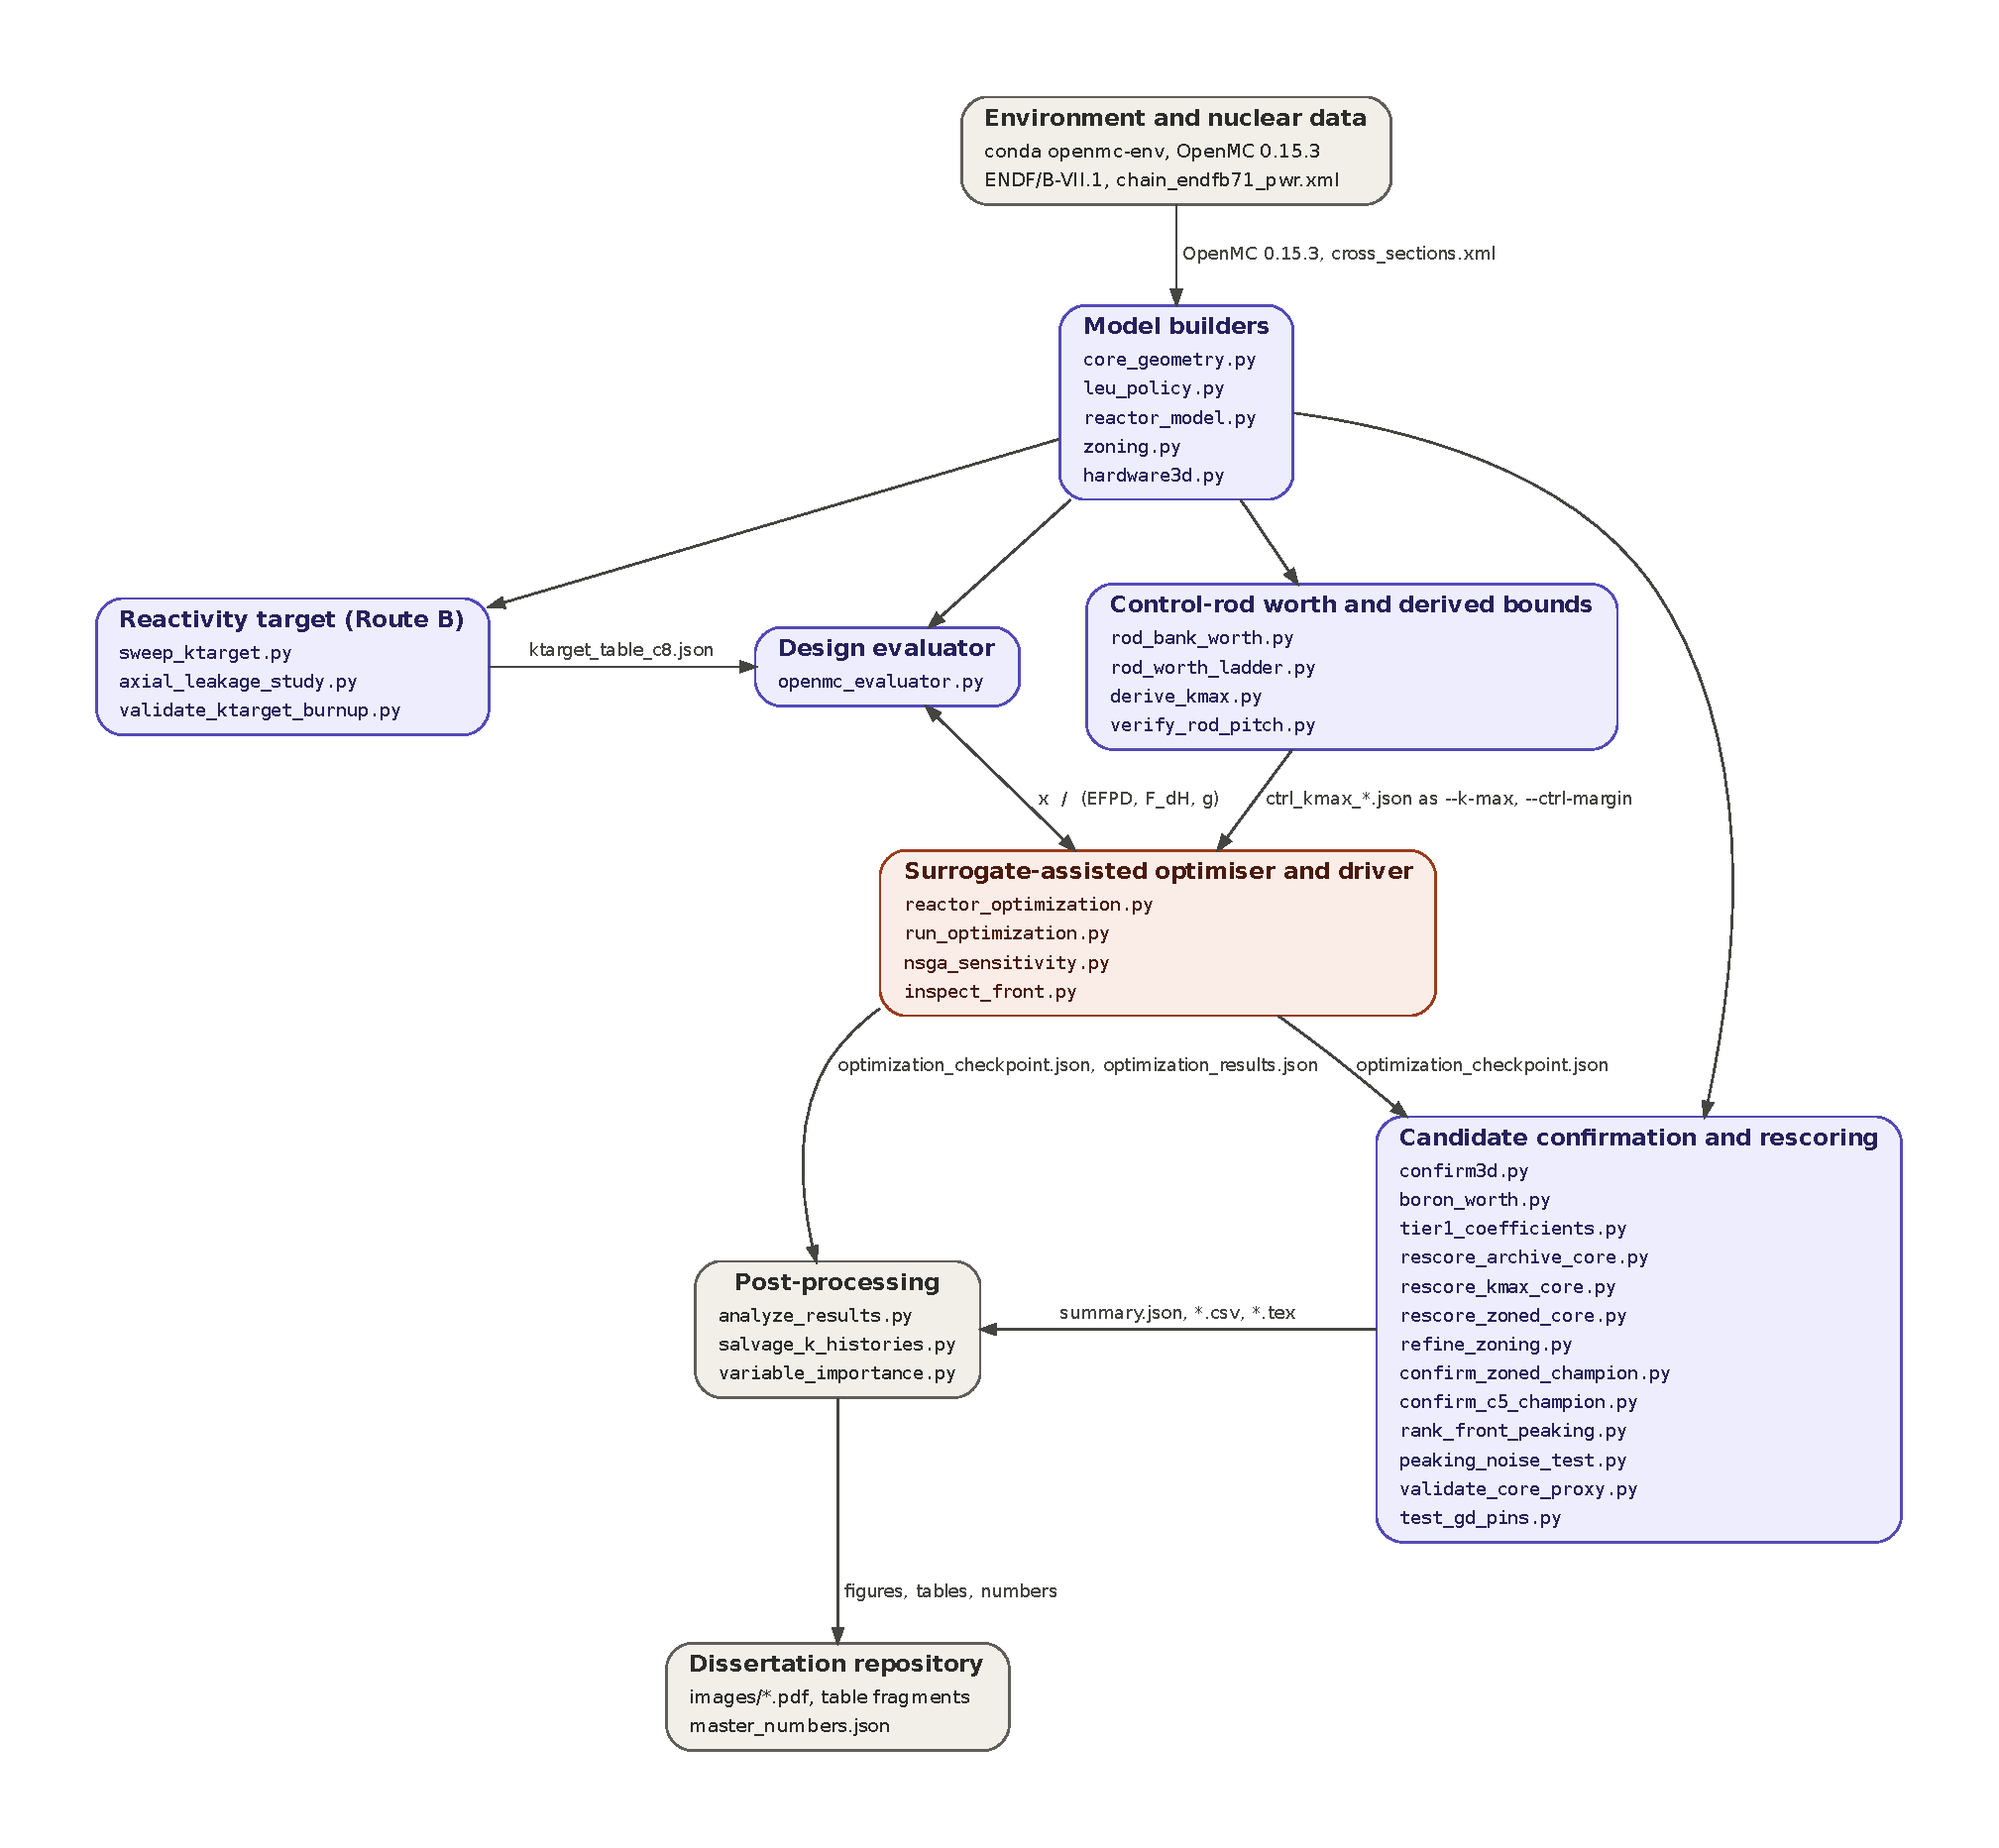
\includegraphics[width=\linewidth]{images/code_architecture.pdf}
  \caption{Macro architecture of the simulation code. Purple blocks run
  OpenMC, the coral block runs the surrogate-assisted optimiser, gray blocks
  are infrastructure and outputs. Scripts listed inside each block are
  detailed in Tables~\ref{tab:arch-builders} to \ref{tab:arch-post}.}
  \label{fig:code-architecture}
\end{figure}

One campaign traverses the blocks in the following order.

\begin{enumerate}[nosep]
  \item The reactivity target table and the derived reactivity ceiling are
        computed once, before the campaign, by the reactivity-target block
        and the control-rod block.
  \item The driver samples the Design of Experiments (DOE) by Latin
        Hypercube Sampling (LHS) \cite{mckay_lhs_1979} and sends each design
        vector to the evaluator.
  \item The evaluator builds the OpenMC models, runs the assembly depletion
        and the core solves, and returns the objectives and the constraint
        vector.
  \item The optimiser fits the Gaussian Process (GP) surrogates
        \cite{rasmussen_gp_2006}, runs the Non-dominated Sorting Genetic
        Algorithm II (NSGA-II) \cite{deb_nsga2_2002} on the surrogates, and
        selects the infill batch. Steps 3 and 4 repeat for each block of
        iterations.
  \item The confirmation block re-evaluates the archived candidates at
        higher fidelity, in three dimensions, and with the control and boron
        studies.
  \item The post-processing block extracts the front, the hypervolume
        history and the corrected depletion histories, and feeds the
        dissertation repository.
\end{enumerate}

\section{Blocks}

\subsection{Environment and nuclear data}

All physics blocks run inside one conda environment, \texttt{openmc-env},
pinned by \texttt{environment.yml} and reproduced in a Docker image by the
\texttt{Dockerfile}. The environment provides OpenMC 0.15.3
\cite{romano_openmc_2015,romano_2021_depletion}, pymoo 0.6.2
\cite{blank_deb_2020} and scikit-learn \cite{pedregosa_sklearn_2011}.

The nuclear data are the ENDF/B-VII.1 continuous-energy cross sections
\cite{chadwick_endf71_2011} and the depletion chain
\file{chain_endfb71_pwr.xml}, downloaded once per machine by
\texttt{setup\_data.sh}. Every script resolves the cross sections through
the environment variable \texttt{OPENMC\_CROSS\_SECTIONS} and the depletion
chain through \texttt{OPENMC\_CHAIN\_FILE}, so no path is written in the
source.

\subsection{Model builders}

This block holds the five library modules that every physics script
imports. They contain no command-line interface and write no result file.
Their outputs are OpenMC model objects, built in memory from a design
dictionary.

\begin{table}[htbp]
  \centering\footnotesize
  \caption{Model builders. These modules are imported, never run.}
  \label{tab:arch-builders}
  \begin{tabularx}{\linewidth}{@{}>{\raggedright\arraybackslash}p{3.6cm} X@{}}
    \toprule
    Module & Role \\
    \midrule
    \file{core_geometry.py} & Vessel envelope, geometric margin, maximum
      reflector thickness, end-of-cycle crossing of the reactivity history,
      bilinear interpolation of the target table \\
    \file{leu_policy.py} & Enrichment cap and search-box constants, defined
      once so that the search box, the evaluator and the driver cannot
      disagree \\
    \file{reactor_model.py} & Materials, fuel pin, guide tube, control-rod
      universes, $17\times17$ assembly and 32-assembly core builders,
      gadolinium pin pattern \\
    \file{zoning.py} & Ring map, centre, middle and periphery multipliers,
      control-bank positions, core beginning-of-life solve, reactivity
      history reader \\
    \file{hardware3d.py} & Finite-height core with the assembly hardware
      stack, used by the three-dimensional confirmation \\
    \bottomrule
  \end{tabularx}
\end{table}

\subsection{Reactivity target (Route B)}

This block produces the end-of-cycle reactivity target used by the
evaluator, as described in the methodology. The target is tabulated on the
full core, corrected for axial leakage, and validated against the burnup
dependence of the leakage.

\begin{table}[htbp]
  \centering\footnotesize
  \caption{Reactivity-target block. The two validation scripts read the
  campaign checkpoint to select the designs they evaluate.}
  \label{tab:arch-ktarget}
  \begin{tabularx}{\linewidth}{@{}>{\raggedright\arraybackslash}p{5.0cm} X >{\raggedright\arraybackslash}p{4.4cm}@{}}
    \toprule
    Script & Role & Main output \\
    \midrule
    \file{sweep_ktarget.py} & Tabulates the target versus pitch and
      reflector thickness from paired assembly and core solves &
      \file{ktarget_table.json} \\
    \file{axial_leakage_study.py} & Axial leakage factor
      $L_{\mathrm{ax}} = k_{2\mathrm{D}}/k_{3\mathrm{D}}$ on archived designs &
      \file{axial_<absorber>.json} \\
    \file{validate_ktarget_burnup.py} & Burnup dependence of the target on
      the front designs & \file{summary.json} \\
    \bottomrule
  \end{tabularx}
\end{table}

\subsection{Design evaluator}

The evaluator is a single module, \file{openmc_evaluator.py}. It is the
only place where a design vector becomes physics. Its public method
\texttt{evaluate\_one} performs three solves per design and returns the
mapping

\[
  \mathbf{x} = \left(e,\, w_{\mathrm{Gd}},\, t_{\mathrm{refl}},\, n_{\mathrm{Gd}}\right)
  \quad\longmapsto\quad
  \left(T_{\mathrm{EFPD}},\, F_{\Delta H},\, \mathbf{g}\right)
\]

\begin{description}[nosep]
  \item[$e$] fuel enrichment, in weight percent of \isotope[235]{U}
  \item[$w_{\mathrm{Gd}}$] gadolinia loading of the poisoned pins, in weight percent
  \item[$t_{\mathrm{refl}}$] radial reflector thickness, in cm
  \item[$n_{\mathrm{Gd}}$] number of poisoned pins per assembly, dimensionless
  \item[$T_{\mathrm{EFPD}}$] cycle length, in effective full power days
  \item[$F_{\Delta H}$] radial enthalpy-rise hot channel factor, dimensionless
  \item[$\mathbf{g}$] constraint vector on reactivity, enrichment and controllability, each entry normalised by its own limit, dimensionless
\end{description}

The three solves are the two-dimensional assembly depletion, which gives
$T_{\mathrm{EFPD}}$ through the end-of-cycle crossing of the target, the
core beginning-of-life solve, which gives $F_{\Delta H}$ and the core
eigenvalue, and the rodded core solve, which gives the controllability
entries of $\mathbf{g}$. The evaluator reads \file{ktarget_table*.json}
and writes one \file{depletion_results.h5} per case.

\subsection{Control-rod worth and derived bounds}

This block measures the worth of the control banks on archived designs and
turns the minimum worth into the reactivity ceiling passed to the driver.
It runs before a campaign, and again on the candidates after it.

\begin{table}[htbp]
  \centering\footnotesize
  \caption{Control-rod block. All scripts read the campaign checkpoint
  except \texttt{derive\_kmax.py}, which reads the screen written by
  \texttt{rod\_bank\_worth.py}.}
  \label{tab:arch-ctrl}
  \begin{tabularx}{\linewidth}{@{}>{\raggedright\arraybackslash}p{5.0cm} X >{\raggedright\arraybackslash}p{4.4cm}@{}}
    \toprule
    Script & Role & Main output \\
    \midrule
    \file{rod_bank_worth.py} & Bank worths and controllability screen of
      archived designs & \file{banks_<absorber>.json} \\
    \file{rod_worth_ladder.py} & Rod-worth ladder and rodded peaking of the
      zoned core & \file{ladder_idx<i>_}\newline\file{<absorber>.json} \\
    \file{derive_kmax.py} & Reactivity ceiling from the minimum bank worth
      and the controllability margin & \file{ctrl_kmax_<group>.json} \\
    \file{verify_rod_pitch.py} & Guide-tube clipping study versus pin pitch &
      \file{fig_rod_pitch_*.pdf} \\
    \bottomrule
  \end{tabularx}
\end{table}

\subsection{Surrogate-assisted optimiser and driver}

The optimiser holds the design space, the surrogates, the acquisition step
and the checkpoint. The driver exposes it as a command line, records the
provenance of every run in the checkpoint, and refuses to resume a
checkpoint whose settings differ from the current command.

\begin{table}[htbp]
  \centering\footnotesize
  \caption{Optimiser block. The driver reads the target table and, on
  resume, the checkpoint. The two analysis scripts read the checkpoint.}
  \label{tab:arch-optimiser}
  \begin{tabularx}{\linewidth}{@{}>{\raggedright\arraybackslash}p{5.0cm} X >{\raggedright\arraybackslash}p{4.4cm}@{}}
    \toprule
    Script & Role & Main output \\
    \midrule
    \file{reactor_optimization.py} & Design space, GP surrogates, NSGA-II
      acquisition on the surrogates, feasibility margin, batch diversity,
      hypervolume, checkpoint & \file{optimization_}\newline\file{checkpoint.json} \\
    \file{run_optimization.py} & Command-line driver: DOE, blocks of infill
      iterations, resume, provenance & \file{optimization_}\newline\file{results.json} \\
    \file{nsga_sensitivity.py} & Sensitivity of the acquisition step to the
      NSGA-II population, generations and seed & \file{nsga_sensitivity.json} \\
    \file{inspect_front.py} & Census of a live checkpoint: front, screens,
      per-block diversity & \file{<prefix>_front.csv} \\
    \bottomrule
  \end{tabularx}
\end{table}

\subsection{Candidate confirmation and rescoring}

This block re-evaluates archived designs outside the optimisation loop. Its
scripts share one pattern. They read the campaign checkpoint, select
designs by index or by front membership, run OpenMC at a fidelity chosen on
the command line, cache every solve in a \file{runs.json} keyed by design
and state, and write a summary. The cache makes every script resumable.

\begin{table}[htbp]
  \centering\footnotesize
  \caption{Confirmation block. All scripts read the campaign checkpoint.}
  \label{tab:arch-confirm}
  \begin{tabularx}{\linewidth}{@{}>{\raggedright\arraybackslash}p{5.0cm} X >{\raggedright\arraybackslash}p{4.4cm}@{}}
    \toprule
    Script & Role & Main output \\
    \midrule
    \file{confirm3d.py} & Three-dimensional confirmation with the hardware
      stack, several rod states and boron concentrations & \file{summary.json} \\
    \file{boron_worth.py} & Boron worth and share of the beginning-of-life
      hold-down across rod states and concentrations & \file{boron_table.tex} \\
    \file{tier1_coefficients.py} & Reactivity coefficients of a candidate &
      \file{tier1_idx<i>.json} \\
    \file{rescore_archive_core.py} & Core-basis peaking of an assembly-basis
      archive & \file{core_rescore.csv} \\
    \file{rescore_kmax_core.py} & Re-screens a finished campaign on the core
      reactivity limits & \file{<label>_kbasis_}\newline\file{summary.json} \\
    \file{rescore_zoned_core.py} & Transfer test of the zoned loading on an
      archive & \file{transfer_summary.json} \\
    \file{refine_zoning.py} & Refinement of the ring multipliers of a
      champion & \file{runs.json} \\
    \file{confirm_zoned_champion.py} & Depletion of the zoned champion at
      full fidelity & \file{confirm_idx<i>.json} \\
    \file{confirm_c5_champion.py} & Feasibility of the Campaign 5 champion
      at full fidelity & \file{summary.json} \\
    \file{rank_front_peaking.py} & Minimum-$F_{\Delta H}$ design beyond
      Monte Carlo noise, by sequential screening & \file{ranking.csv} \\
    \file{peaking_noise_test.py} & Seed replicates of $F_{\Delta H}$ on the
      front designs & \file{noise_summary.csv} \\
    \file{validate_core_proxy.py} & Assembly-to-core peaking proxy
      validation & \file{core_validation.csv} \\
    \file{test_gd_pins.py} & Gadolinium pin-count test on a champion,
      assembly and core & \file{summary.json} \\
    \bottomrule
  \end{tabularx}
\end{table}

\subsection{Post-processing}

The post-processing block reads the campaign archive and the confirmation
summaries and produces the quantities reported in the results chapters.

\begin{table}[htbp]
  \centering\footnotesize
  \caption{Post-processing block. Figure generators and log parsers are
  omitted, see Section~\ref{sec:arch-scope}.}
  \label{tab:arch-post}
  \begin{tabularx}{\linewidth}{@{}>{\raggedright\arraybackslash}p{5.0cm} X >{\raggedright\arraybackslash}p{4.4cm}@{}}
    \toprule
    Script & Role & Main output \\
    \midrule
    \file{analyze_results.py} & Pareto front, hypervolume history,
      design-space diagnostics & figures \\
    \file{salvage_k_histories.py} & Corrects the archived depletion histories
      for the restart defect of the depletion chunks & \file{salvage_summary.csv} \\
    \file{variable_importance.py} & Permutation importance of the design
      variables on the archive & standard output \\
    \bottomrule
  \end{tabularx}
\end{table}

\subsection{Dissertation repository}

The dissertation is kept in a second repository,
\url{https://github.com/dcrlopes/Masther-Thesis-UNIPI---Di-go-Lopes},
synchronised with Overleaf. Figures are stored under \texttt{images/}.
Every number quoted in the text is taken from
\file{master_numbers.json}, which is the single source of truth for the
thesis.

\openpoint{\file{master_numbers.json} is not under version control in
either repository. It was produced with the computational-cost section and
lives only on the workstation. Commit it to \texttt{results\_timing/} in the
simulation repository before submission, so that the last arrow of
Figure~\ref{fig:code-architecture} points to a file a reader can open.}

\section{Interfaces between blocks}

Table~\ref{tab:arch-interfaces} lists the artefacts that cross the block
boundaries of Figure~\ref{fig:code-architecture}. Every artefact is a
plain text file, JSON or CSV, so that any stage can be inspected without
the code.

\begin{table}[htbp]
  \centering\footnotesize
  \caption{Artefacts exchanged between blocks.}
  \label{tab:arch-interfaces}
  \begin{tabularx}{\linewidth}{@{}>{\raggedright\arraybackslash}p{5.1cm} >{\raggedright\arraybackslash}p{2.1cm} >{\raggedright\arraybackslash}p{2.5cm} X@{}}
    \toprule
    Artefact & Producer & Consumer & Content \\
    \midrule
    \file{ktarget_table_c8.json} & Reactivity target & Evaluator &
      Target $k$ versus pitch and reflector thickness, with the axial
      correction $L_{\mathrm{ax}}$ \\
    \file{ctrl_kmax_<group>.json} & Control-rod worth & Driver &
      Derived ceiling, passed as \texttt{--k-max} and \texttt{--ctrl-margin} \\
    design vector $\mathbf{x}$ & Optimiser & Evaluator &
      One design per call \\
    $(T_{\mathrm{EFPD}}, F_{\Delta H}, \mathbf{g})$ & Evaluator & Optimiser &
      Objectives and normalised constraints \\
    \file{optimization_checkpoint.json} & Optimiser & Confirmation,
      post-processing & Every evaluation of the campaign with its
      provenance \\
    \file{optimization_results.json} & Optimiser & Post-processing &
      Front, raw objectives, hypervolume history \\
    \file{summary.json}, \file{*.csv} & Confirmation & Post-processing &
      Per-design results of each confirmation study \\
    \file{images/*.pdf}, \file{*.tex} & Post-processing & Dissertation &
      Figures and table fragments \\
    \bottomrule
  \end{tabularx}
\end{table}

The checkpoint is the central artefact. It is written at the end of every
block of iterations and it records the design space, the constraint
definition, the transport fidelity, the target table and the command line.
A resumed run compares these fields with its own arguments and warns on any
difference. All confirmation and post-processing scripts read the
checkpoint, never the raw case directories, so a campaign can be
re-analysed from a single file.

\openpoint{Regenerate the table of Section~1 of the repository
\texttt{README.md} with \texttt{make\_architecture\_figure.py --table md},
because the current table describes the Campaign 3 layout.}
                       (add this line)
%%   \end{appendices}
%%
%% Figure: images/code_architecture.pdf, produced by
%% make_architecture_figure.py in the simulation repository. Regenerate the
%% figure and the table rows (--table latex) whenever a script is added.
%%
%% New bibliography entries required (appended to references_additions.bib):
%%   pedregosa_sklearn_2011, chadwick_endf71_2011
%% ---------------------------------------------------------------------

\chapter{Architecture of the simulation code}\label{app:code-architecture}

\providecommand{\file}[1]{\texttt{\detokenize{#1}}}

\providecommand{\openpoint}[1]{\par\noindent\fbox{\parbox{0.97\linewidth}{%
  \small\textbf{Open point.} #1}}\par}

\section{Purpose and scope}\label{sec:arch-scope}

This appendix documents the organisation of the code that produced every
result in this thesis. It is written for a reader who needs to locate the
script behind a number, reproduce a campaign, or extend the pipeline to
another core.

The code is public. It is hosted at
\url{https://github.com/dcrlopes/master-thesis-unipi}, on the branch
\texttt{campaign8}, which is the state used for the final campaign and for
the candidate confirmation runs. The state described in this appendix is
commit \texttt{22bad3d} of 3 September 2026.

\openpoint{Update the commit hash above to the final state of branch
\texttt{campaign8} at submission. The branch \texttt{main} still holds the
Campaign 3 state of the code and must not be cited.}

The repository contains 92 Python scripts and 8 shell wrappers. Only the
scripts that perform a computation reported in the thesis are described
here. The following groups are omitted on purpose.

\begin{itemize}[nosep]
  \item Shell wrappers for launch, resume and monitoring.
  \item Anchor-verified patch scripts (\texttt{apply\_*.py},
        \texttt{fix\_*.py}, \texttt{repair\_*.py}) that modified the source
        between campaigns. Their role is described in the methodology.
  \item Figure generators, log parsers and timing accounting scripts.
  \item Unit tests, diagnostics and scripts superseded by a later version.
\end{itemize}

\section{Macro architecture}

Figure~\ref{fig:code-architecture} shows the nine blocks of the pipeline and
the artefacts that cross each interface. Purple blocks call OpenMC
\cite{romano_openmc_2015}, the Monte Carlo transport and depletion code.
The coral block is the only one that never calls OpenMC directly. Gray
blocks are infrastructure and outputs. Unlabelled arrows are Python
imports. Labelled arrows name the file, or the pair of vectors, exchanged.

\begin{figure}[htbp]
  \centering
  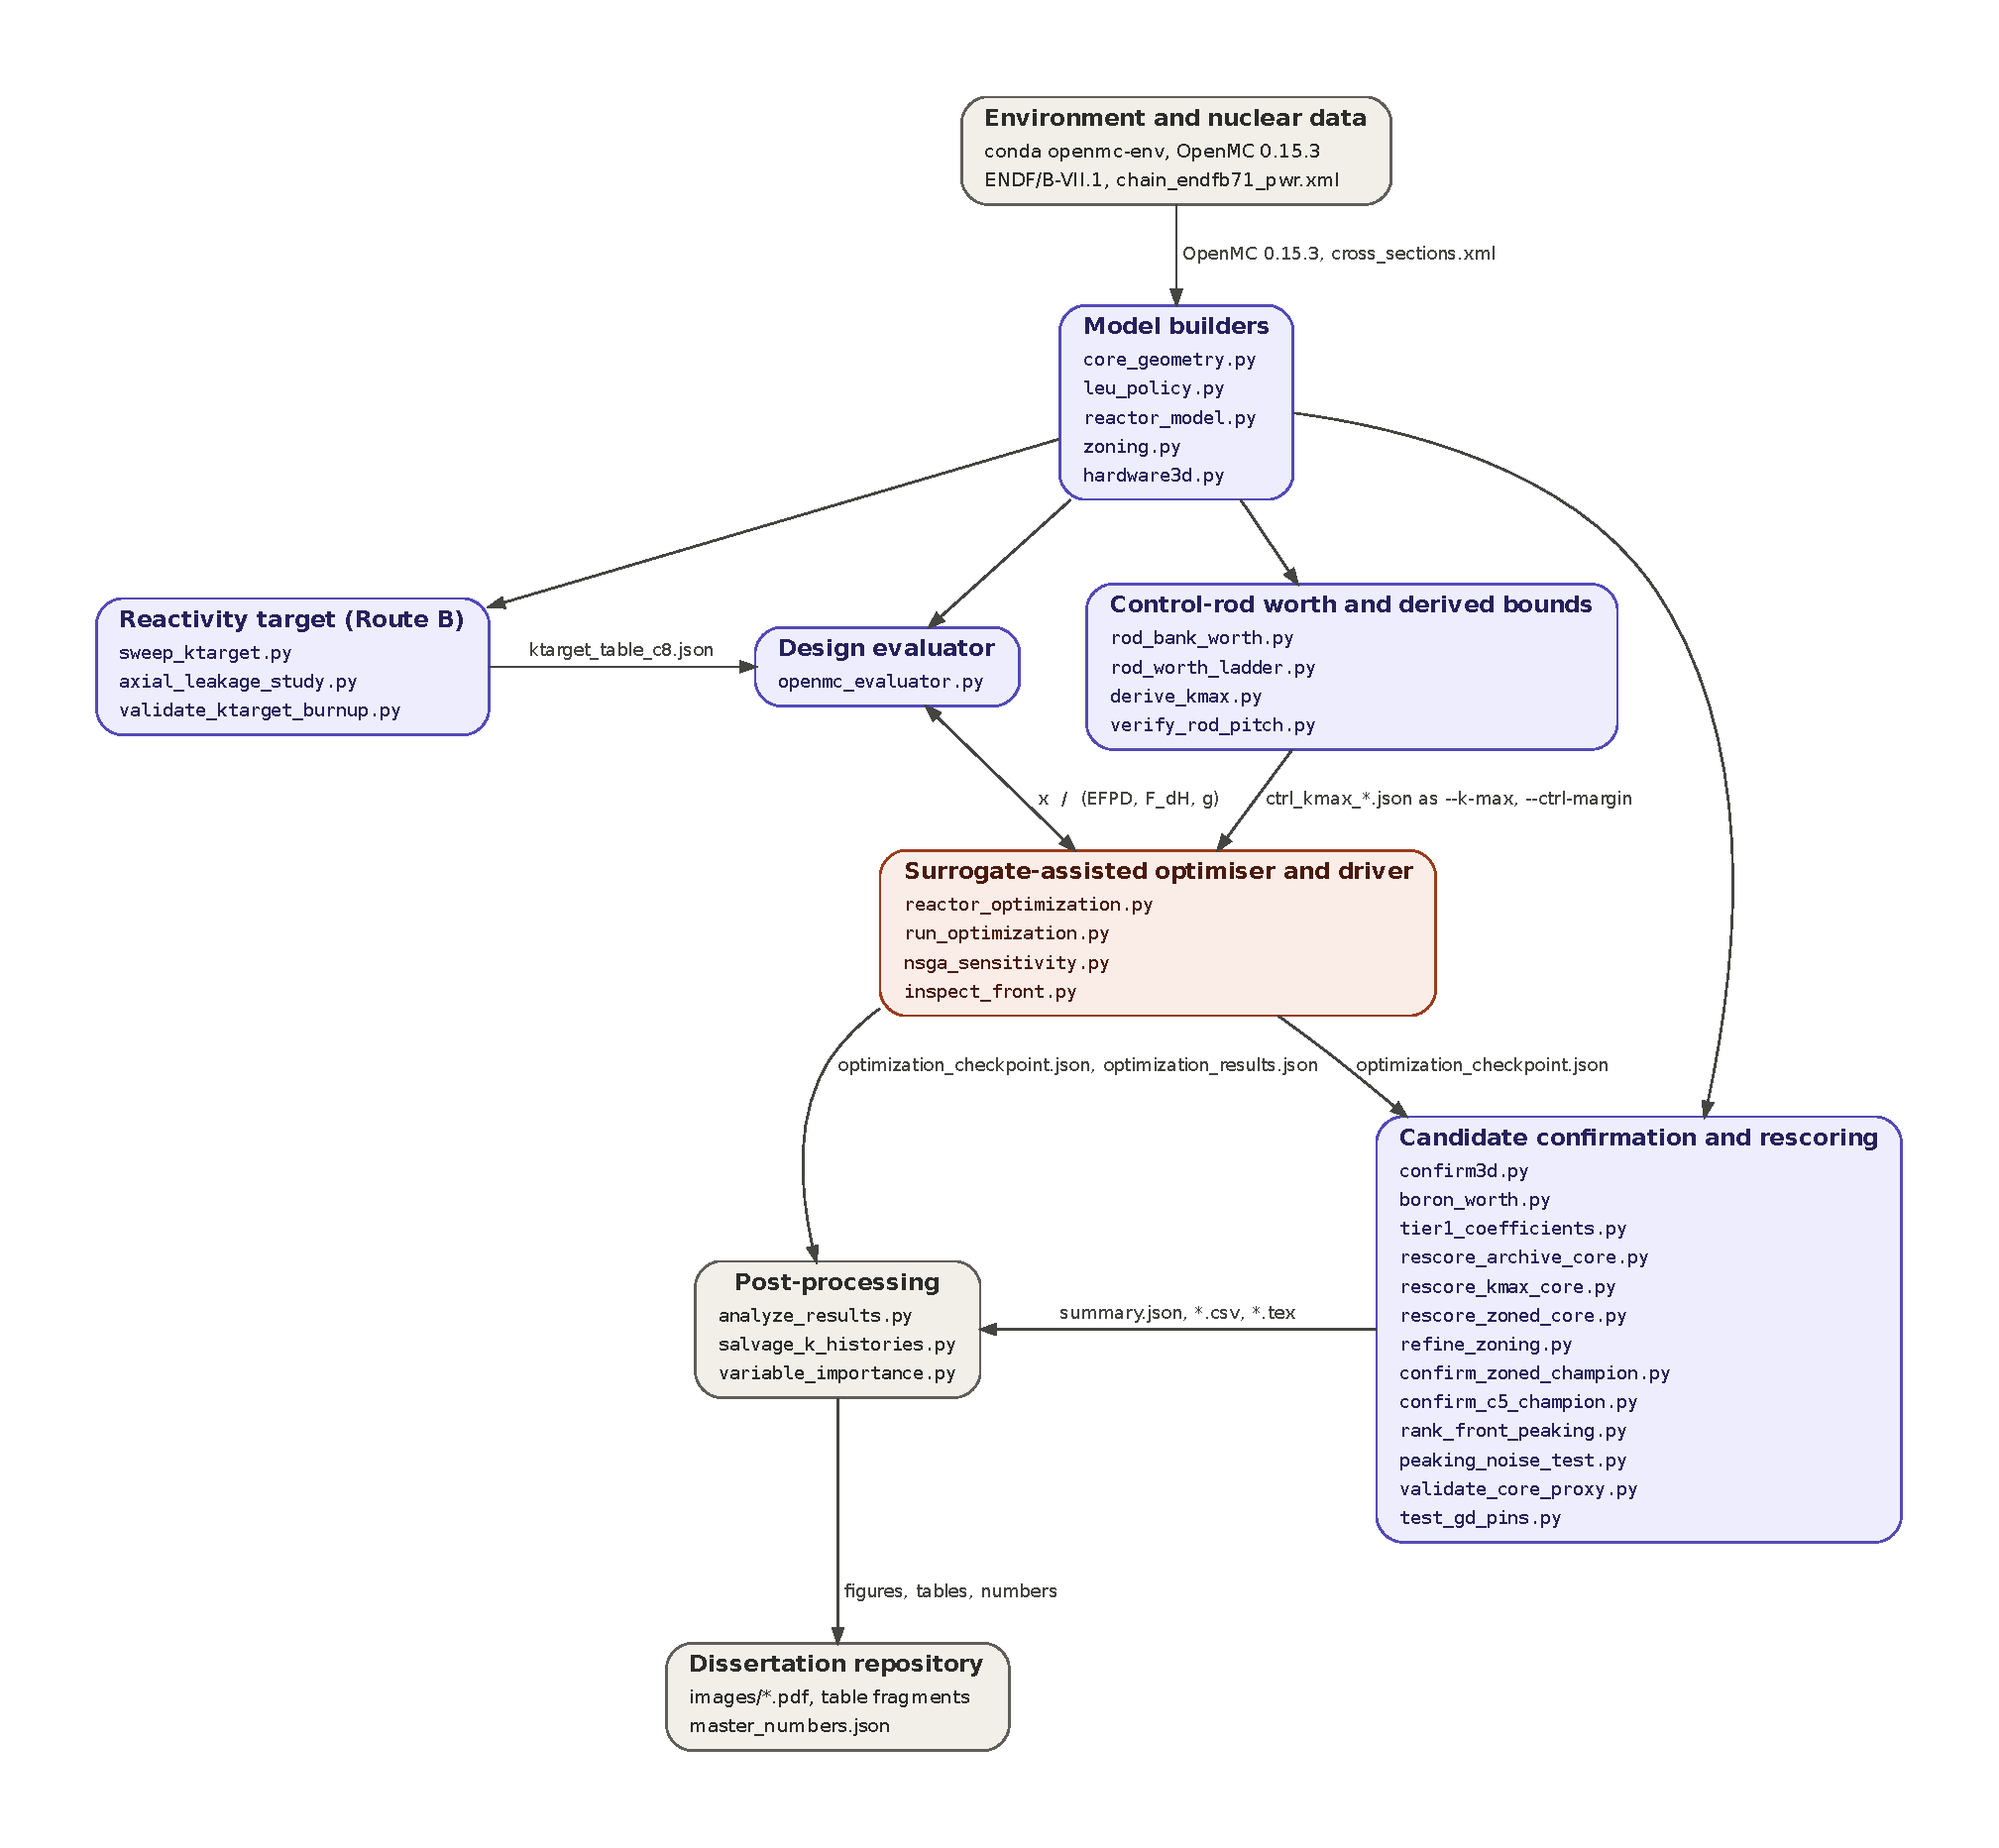
\includegraphics[width=\linewidth]{images/code_architecture.pdf}
  \caption{Macro architecture of the simulation code. Purple blocks run
  OpenMC, the coral block runs the surrogate-assisted optimiser, gray blocks
  are infrastructure and outputs. Scripts listed inside each block are
  detailed in Tables~\ref{tab:arch-builders} to \ref{tab:arch-post}.}
  \label{fig:code-architecture}
\end{figure}

One campaign traverses the blocks in the following order.

\begin{enumerate}[nosep]
  \item The reactivity target table and the derived reactivity ceiling are
        computed once, before the campaign, by the reactivity-target block
        and the control-rod block.
  \item The driver samples the Design of Experiments (DOE) by Latin
        Hypercube Sampling (LHS) \cite{mckay_lhs_1979} and sends each design
        vector to the evaluator.
  \item The evaluator builds the OpenMC models, runs the assembly depletion
        and the core solves, and returns the objectives and the constraint
        vector.
  \item The optimiser fits the Gaussian Process (GP) surrogates
        \cite{rasmussen_gp_2006}, runs the Non-dominated Sorting Genetic
        Algorithm II (NSGA-II) \cite{deb_nsga2_2002} on the surrogates, and
        selects the infill batch. Steps 3 and 4 repeat for each block of
        iterations.
  \item The confirmation block re-evaluates the archived candidates at
        higher fidelity, in three dimensions, and with the control and boron
        studies.
  \item The post-processing block extracts the front, the hypervolume
        history and the corrected depletion histories, and feeds the
        dissertation repository.
\end{enumerate}

\section{Blocks}

\subsection{Environment and nuclear data}

All physics blocks run inside one conda environment, \texttt{openmc-env},
pinned by \texttt{environment.yml} and reproduced in a Docker image by the
\texttt{Dockerfile}. The environment provides OpenMC 0.15.3
\cite{romano_openmc_2015,romano_2021_depletion}, pymoo 0.6.2
\cite{blank_deb_2020} and scikit-learn \cite{pedregosa_sklearn_2011}.

The nuclear data are the ENDF/B-VII.1 continuous-energy cross sections
\cite{chadwick_endf71_2011} and the depletion chain
\file{chain_endfb71_pwr.xml}, downloaded once per machine by
\texttt{setup\_data.sh}. Every script resolves the cross sections through
the environment variable \texttt{OPENMC\_CROSS\_SECTIONS} and the depletion
chain through \texttt{OPENMC\_CHAIN\_FILE}, so no path is written in the
source.

\subsection{Model builders}

This block holds the five library modules that every physics script
imports. They contain no command-line interface and write no result file.
Their outputs are OpenMC model objects, built in memory from a design
dictionary.

\begin{table}[htbp]
  \centering\footnotesize
  \caption{Model builders. These modules are imported, never run.}
  \label{tab:arch-builders}
  \begin{tabularx}{\linewidth}{@{}>{\raggedright\arraybackslash}p{3.6cm} X@{}}
    \toprule
    Module & Role \\
    \midrule
    \file{core_geometry.py} & Vessel envelope, geometric margin, maximum
      reflector thickness, end-of-cycle crossing of the reactivity history,
      bilinear interpolation of the target table \\
    \file{leu_policy.py} & Enrichment cap and search-box constants, defined
      once so that the search box, the evaluator and the driver cannot
      disagree \\
    \file{reactor_model.py} & Materials, fuel pin, guide tube, control-rod
      universes, $17\times17$ assembly and 32-assembly core builders,
      gadolinium pin pattern \\
    \file{zoning.py} & Ring map, centre, middle and periphery multipliers,
      control-bank positions, core beginning-of-life solve, reactivity
      history reader \\
    \file{hardware3d.py} & Finite-height core with the assembly hardware
      stack, used by the three-dimensional confirmation \\
    \bottomrule
  \end{tabularx}
\end{table}

\subsection{Reactivity target (Route B)}

This block produces the end-of-cycle reactivity target used by the
evaluator, as described in the methodology. The target is tabulated on the
full core, corrected for axial leakage, and validated against the burnup
dependence of the leakage.

\begin{table}[htbp]
  \centering\footnotesize
  \caption{Reactivity-target block. The two validation scripts read the
  campaign checkpoint to select the designs they evaluate.}
  \label{tab:arch-ktarget}
  \begin{tabularx}{\linewidth}{@{}>{\raggedright\arraybackslash}p{5.0cm} X >{\raggedright\arraybackslash}p{4.4cm}@{}}
    \toprule
    Script & Role & Main output \\
    \midrule
    \file{sweep_ktarget.py} & Tabulates the target versus pitch and
      reflector thickness from paired assembly and core solves &
      \file{ktarget_table.json} \\
    \file{axial_leakage_study.py} & Axial leakage factor
      $L_{\mathrm{ax}} = k_{2\mathrm{D}}/k_{3\mathrm{D}}$ on archived designs &
      \file{axial_<absorber>.json} \\
    \file{validate_ktarget_burnup.py} & Burnup dependence of the target on
      the front designs & \file{summary.json} \\
    \bottomrule
  \end{tabularx}
\end{table}

\subsection{Design evaluator}

The evaluator is a single module, \file{openmc_evaluator.py}. It is the
only place where a design vector becomes physics. Its public method
\texttt{evaluate\_one} performs three solves per design and returns the
mapping

\[
  \mathbf{x} = \left(e,\, w_{\mathrm{Gd}},\, t_{\mathrm{refl}},\, n_{\mathrm{Gd}}\right)
  \quad\longmapsto\quad
  \left(T_{\mathrm{EFPD}},\, F_{\Delta H},\, \mathbf{g}\right)
\]

\begin{description}[nosep]
  \item[$e$] fuel enrichment, in weight percent of \isotope[235]{U}
  \item[$w_{\mathrm{Gd}}$] gadolinia loading of the poisoned pins, in weight percent
  \item[$t_{\mathrm{refl}}$] radial reflector thickness, in cm
  \item[$n_{\mathrm{Gd}}$] number of poisoned pins per assembly, dimensionless
  \item[$T_{\mathrm{EFPD}}$] cycle length, in effective full power days
  \item[$F_{\Delta H}$] radial enthalpy-rise hot channel factor, dimensionless
  \item[$\mathbf{g}$] constraint vector on reactivity, enrichment and controllability, each entry normalised by its own limit, dimensionless
\end{description}

The three solves are the two-dimensional assembly depletion, which gives
$T_{\mathrm{EFPD}}$ through the end-of-cycle crossing of the target, the
core beginning-of-life solve, which gives $F_{\Delta H}$ and the core
eigenvalue, and the rodded core solve, which gives the controllability
entries of $\mathbf{g}$. The evaluator reads \file{ktarget_table*.json}
and writes one \file{depletion_results.h5} per case.

\subsection{Control-rod worth and derived bounds}

This block measures the worth of the control banks on archived designs and
turns the minimum worth into the reactivity ceiling passed to the driver.
It runs before a campaign, and again on the candidates after it.

\begin{table}[htbp]
  \centering\footnotesize
  \caption{Control-rod block. All scripts read the campaign checkpoint
  except \texttt{derive\_kmax.py}, which reads the screen written by
  \texttt{rod\_bank\_worth.py}.}
  \label{tab:arch-ctrl}
  \begin{tabularx}{\linewidth}{@{}>{\raggedright\arraybackslash}p{5.0cm} X >{\raggedright\arraybackslash}p{4.4cm}@{}}
    \toprule
    Script & Role & Main output \\
    \midrule
    \file{rod_bank_worth.py} & Bank worths and controllability screen of
      archived designs & \file{banks_<absorber>.json} \\
    \file{rod_worth_ladder.py} & Rod-worth ladder and rodded peaking of the
      zoned core & \file{ladder_idx<i>_}\newline\file{<absorber>.json} \\
    \file{derive_kmax.py} & Reactivity ceiling from the minimum bank worth
      and the controllability margin & \file{ctrl_kmax_<group>.json} \\
    \file{verify_rod_pitch.py} & Guide-tube clipping study versus pin pitch &
      \file{fig_rod_pitch_*.pdf} \\
    \bottomrule
  \end{tabularx}
\end{table}

\subsection{Surrogate-assisted optimiser and driver}

The optimiser holds the design space, the surrogates, the acquisition step
and the checkpoint. The driver exposes it as a command line, records the
provenance of every run in the checkpoint, and refuses to resume a
checkpoint whose settings differ from the current command.

\begin{table}[htbp]
  \centering\footnotesize
  \caption{Optimiser block. The driver reads the target table and, on
  resume, the checkpoint. The two analysis scripts read the checkpoint.}
  \label{tab:arch-optimiser}
  \begin{tabularx}{\linewidth}{@{}>{\raggedright\arraybackslash}p{5.0cm} X >{\raggedright\arraybackslash}p{4.4cm}@{}}
    \toprule
    Script & Role & Main output \\
    \midrule
    \file{reactor_optimization.py} & Design space, GP surrogates, NSGA-II
      acquisition on the surrogates, feasibility margin, batch diversity,
      hypervolume, checkpoint & \file{optimization_}\newline\file{checkpoint.json} \\
    \file{run_optimization.py} & Command-line driver: DOE, blocks of infill
      iterations, resume, provenance & \file{optimization_}\newline\file{results.json} \\
    \file{nsga_sensitivity.py} & Sensitivity of the acquisition step to the
      NSGA-II population, generations and seed & \file{nsga_sensitivity.json} \\
    \file{inspect_front.py} & Census of a live checkpoint: front, screens,
      per-block diversity & \file{<prefix>_front.csv} \\
    \bottomrule
  \end{tabularx}
\end{table}

\subsection{Candidate confirmation and rescoring}

This block re-evaluates archived designs outside the optimisation loop. Its
scripts share one pattern. They read the campaign checkpoint, select
designs by index or by front membership, run OpenMC at a fidelity chosen on
the command line, cache every solve in a \file{runs.json} keyed by design
and state, and write a summary. The cache makes every script resumable.

\begin{table}[htbp]
  \centering\footnotesize
  \caption{Confirmation block. All scripts read the campaign checkpoint.}
  \label{tab:arch-confirm}
  \begin{tabularx}{\linewidth}{@{}>{\raggedright\arraybackslash}p{5.0cm} X >{\raggedright\arraybackslash}p{4.4cm}@{}}
    \toprule
    Script & Role & Main output \\
    \midrule
    \file{confirm3d.py} & Three-dimensional confirmation with the hardware
      stack, several rod states and boron concentrations & \file{summary.json} \\
    \file{boron_worth.py} & Boron worth and share of the beginning-of-life
      hold-down across rod states and concentrations & \file{boron_table.tex} \\
    \file{tier1_coefficients.py} & Reactivity coefficients of a candidate &
      \file{tier1_idx<i>.json} \\
    \file{rescore_archive_core.py} & Core-basis peaking of an assembly-basis
      archive & \file{core_rescore.csv} \\
    \file{rescore_kmax_core.py} & Re-screens a finished campaign on the core
      reactivity limits & \file{<label>_kbasis_}\newline\file{summary.json} \\
    \file{rescore_zoned_core.py} & Transfer test of the zoned loading on an
      archive & \file{transfer_summary.json} \\
    \file{refine_zoning.py} & Refinement of the ring multipliers of a
      champion & \file{runs.json} \\
    \file{confirm_zoned_champion.py} & Depletion of the zoned champion at
      full fidelity & \file{confirm_idx<i>.json} \\
    \file{confirm_c5_champion.py} & Feasibility of the Campaign 5 champion
      at full fidelity & \file{summary.json} \\
    \file{rank_front_peaking.py} & Minimum-$F_{\Delta H}$ design beyond
      Monte Carlo noise, by sequential screening & \file{ranking.csv} \\
    \file{peaking_noise_test.py} & Seed replicates of $F_{\Delta H}$ on the
      front designs & \file{noise_summary.csv} \\
    \file{validate_core_proxy.py} & Assembly-to-core peaking proxy
      validation & \file{core_validation.csv} \\
    \file{test_gd_pins.py} & Gadolinium pin-count test on a champion,
      assembly and core & \file{summary.json} \\
    \bottomrule
  \end{tabularx}
\end{table}

\subsection{Post-processing}

The post-processing block reads the campaign archive and the confirmation
summaries and produces the quantities reported in the results chapters.

\begin{table}[htbp]
  \centering\footnotesize
  \caption{Post-processing block. Figure generators and log parsers are
  omitted, see Section~\ref{sec:arch-scope}.}
  \label{tab:arch-post}
  \begin{tabularx}{\linewidth}{@{}>{\raggedright\arraybackslash}p{5.0cm} X >{\raggedright\arraybackslash}p{4.4cm}@{}}
    \toprule
    Script & Role & Main output \\
    \midrule
    \file{analyze_results.py} & Pareto front, hypervolume history,
      design-space diagnostics & figures \\
    \file{salvage_k_histories.py} & Corrects the archived depletion histories
      for the restart defect of the depletion chunks & \file{salvage_summary.csv} \\
    \file{variable_importance.py} & Permutation importance of the design
      variables on the archive & standard output \\
    \bottomrule
  \end{tabularx}
\end{table}

\subsection{Dissertation repository}

The dissertation is kept in a second repository,
\url{https://github.com/dcrlopes/Masther-Thesis-UNIPI---Di-go-Lopes},
synchronised with Overleaf. Figures are stored under \texttt{images/}.
Every number quoted in the text is taken from
\file{master_numbers.json}, which is the single source of truth for the
thesis.

\openpoint{\file{master_numbers.json} is not under version control in
either repository. It was produced with the computational-cost section and
lives only on the workstation. Commit it to \texttt{results\_timing/} in the
simulation repository before submission, so that the last arrow of
Figure~\ref{fig:code-architecture} points to a file a reader can open.}

\section{Interfaces between blocks}

Table~\ref{tab:arch-interfaces} lists the artefacts that cross the block
boundaries of Figure~\ref{fig:code-architecture}. Every artefact is a
plain text file, JSON or CSV, so that any stage can be inspected without
the code.

\begin{table}[htbp]
  \centering\footnotesize
  \caption{Artefacts exchanged between blocks.}
  \label{tab:arch-interfaces}
  \begin{tabularx}{\linewidth}{@{}>{\raggedright\arraybackslash}p{5.1cm} >{\raggedright\arraybackslash}p{2.1cm} >{\raggedright\arraybackslash}p{2.5cm} X@{}}
    \toprule
    Artefact & Producer & Consumer & Content \\
    \midrule
    \file{ktarget_table_c8.json} & Reactivity target & Evaluator &
      Target $k$ versus pitch and reflector thickness, with the axial
      correction $L_{\mathrm{ax}}$ \\
    \file{ctrl_kmax_<group>.json} & Control-rod worth & Driver &
      Derived ceiling, passed as \texttt{--k-max} and \texttt{--ctrl-margin} \\
    design vector $\mathbf{x}$ & Optimiser & Evaluator &
      One design per call \\
    $(T_{\mathrm{EFPD}}, F_{\Delta H}, \mathbf{g})$ & Evaluator & Optimiser &
      Objectives and normalised constraints \\
    \file{optimization_checkpoint.json} & Optimiser & Confirmation,
      post-processing & Every evaluation of the campaign with its
      provenance \\
    \file{optimization_results.json} & Optimiser & Post-processing &
      Front, raw objectives, hypervolume history \\
    \file{summary.json}, \file{*.csv} & Confirmation & Post-processing &
      Per-design results of each confirmation study \\
    \file{images/*.pdf}, \file{*.tex} & Post-processing & Dissertation &
      Figures and table fragments \\
    \bottomrule
  \end{tabularx}
\end{table}

The checkpoint is the central artefact. It is written at the end of every
block of iterations and it records the design space, the constraint
definition, the transport fidelity, the target table and the command line.
A resumed run compares these fields with its own arguments and warns on any
difference. All confirmation and post-processing scripts read the
checkpoint, never the raw case directories, so a campaign can be
re-analysed from a single file.

\openpoint{Regenerate the table of Section~1 of the repository
\texttt{README.md} with \texttt{make\_architecture\_figure.py --table md},
because the current table describes the Campaign 3 layout.}
